\section{Solução Implementada}

    O aplicativo Encontre na UFMS foi desenvolvido com o intuito de facilitar a navegação pelo campus da UFMS em Campo Grande, permitindo que usuários encontrem e localizem pontos de interesse dentro do campus, estes sendo cadastrados por outros usuários, possibilitando que locais que não estão presentes em outros aplicativos de localização sejam documentados e compartilhados com a comunidade acadêmica. Os usuários também terão poder de avaliar os locais cadastrados, podendo assim, ajudar outros usuários a escolherem o melhor local para suas necessidades.

\subsection{Análise Crítica e contribuição do Encontre na UFMS}
    Para podermos analisar o diferencial do aplicativo Encontre na UFMS podemos compará-lo com os aplicativos Google Maps e Localização UFMS. O Google Maps é um aplicativo de geolocalização muito utilizado no mundo todo, porém, ele não é focado em um local específico, como o campus da UFMS, e sim em todo o mundo, sendo assim ele não possui registrado diversos locais de menor escala mas que podem ser de grande importância para algum visitante ou alunos. Já o Localização UFMS é um aplicativo web que disponibiliza um mapa interativo da UFMS que possui mais de 2900 pontos de interesse registrados, porém, ele não possui alguns pontos de interesse que podem ser de grande importância para a comunidade acadêmica, como por exemplo, o Restaurante Universitário e também não informa ao usuário como chegar até o local desejado já que ele é focado em apenas mostrar informações sobre um certo local, ele também não tem fotos de todos os locais e não é colaborativo uma vez que apenas a administração da UFMS pode adicionar novos locais.

\newpage

\subsection{Comparação entre o Encontre na UFMS e outros aplicativos}
    A Tabela 1 apresenta uma comparação entre os aplicativos Google Maps, Localização UFMS e Encontre na UFMS, destacando as principais características de cada aplicativo.

\begin{table}[h]
    \begin{tabularx}{\textwidth}{|X|X|X|X|}
        \hline
        \textbf{Características} & \textbf{Google Maps} & \textbf{Localização UFMS} & \textbf{Encontre na UFMS} \\ \hline
        \textbf{Objetivo Principal} & Geolocalização global & Mapa interativo da UFMS & Navegação pelo campus da UFMS \\ \hline
        \textbf{Público-Alvo} & Usuários em geral & Comunidade acadêmica da UFMS & Comunidade acadêmica da UFMS \\ \hline
        \textbf{Principais Funcionalidades} & Busca de locais, rotas, informações de contato, horários de funcionamento & Busca de locais no campus, informações sobre pontos de interesse & Busca de locais, rotas, cadastro colaborativo de locais, avaliações de locais \\ \hline
    \end{tabularx}
    \caption{Comparação entre aplicativos de localização}
    \label{tab:comparacao-aplicativos}
\end{table}

\subsection{Implementação}

    O desenvolvimento do aplicativo Encontre na UFMS foi dividido em duas partes principais: o backend e o frontend. Trataremos a seguir de cada uma dessas partes, detalhando as tecnologias utilizadas e as funcionalidades implementadas.

\subsubsection{Frontend}

    O frontend foi desenvolvido utilizando o framework Flutter, que permite o desenvolvimento de aplicativos móveis para Android e iOS a partir de um único código fonte. O Flutter é uma ferramenta moderna e de fácil utilização, que permite a criação de interfaces de usuário atraentes e responsivas.

    O código foi desenvolvido com base na \textit{Clean Architecture} \cite{cleanarchitecture}, que é um padrão de arquitetura de software que visa separar as responsabilidades do código em camadas bem definidas, facilitando a manutenção e a evolução do sistema. A arquitetura do aplicativo foi dividida em três camadas principais: a camada de apresentação, a camada de domínio e a camada de dados. A camada de apresentação é responsável por exibir os dados para o usuário e capturar as interações do usuário com o sistema. A camada de domínio contém as regras de negócio do sistema, enquanto a camada de dados é responsável por acessar os dados do sistema, seja de um banco de dados local ou de uma API remota. Essa divisão de camadas é ilustrada na Figura 1.

    \begin{figure}[h]
        \centering
        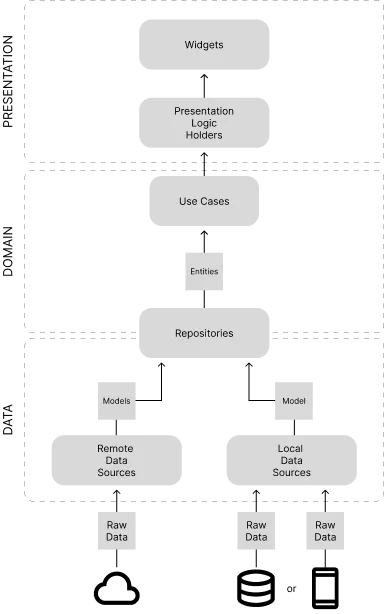
\includegraphics[width=44mm,height=80mm]{imagens/cleanarch.png}
        \caption{\scriptsize Clean Architecture}
        \footnotesize  \centering{\textbf{Fonte: Semih Altin\cite{cleanarchitecture}}}
        \label{fig:clean-architecture}
    \end{figure}

    \FloatBarrier

    Embora o Flutter seja capaz de gerar aplicativos nativos para Android e iOS, o aplicativo Encontre na UFMS foi desenvolvido apenas para Android, visto que a Apple, dona do sistema operacional iOS, restringe o desenvolvimento para seu sistema caso o desenvolvedor não possua um dispositivo da marca. Mas, em teoria, o aplicativo poderia ser facilmente adaptado para iOS, bastando apenas compilar o código fonte em um ambiente de desenvolvimento da Apple. O código-fonte do frontend está disponível no repositório em: \textit{Frontend Encontre Na Ufms} \cite{frontend}.

\subsubsection{Backend}

    O backend foi desenvolvido utilizando o framework Fastify, a fim de garantir excelente desempenho mesmo com um grande volume de requisições, permitindo escalabilidade sem perder a segurança. Foi programado utilizando o Node.js, uma ferramenta que permite a execução de código JavaScript em um ambiente fora do navegador, com excelente desempenho e confiabilidade. 
    
    Durante o desenvolvimento, foi utilizado a linguagem de programação Typescript para tipagem de variáveis, classes e objetos, evitando eventuais erros que poderiam ser causados por incompatibilidade de tipos. Para a execução do código utilizando o Node.js, foi utilizado uma ferramenta do TypeScript: "tsc" ou TypeScript Compiler, para transpilação do código-fonte em JavaScript durante o desenvolvimento, enquanto que para ser utilizado em produção, foi utilizado o tsup, uma ferramenta de empacotamento e transpilação de código TypeScript para JavaScript, rápida e eficiente.

    O código foi desenvolvido utilizando o padrão de software \textit{MVC ou Model-View-Controller} \cite{mvc}, sendo em português: Modelo-Visão-Controlador. As três camadas se entrelaçam entre si, onde o Controlador recebe as requisições do usuário e as envia para o Modelo, que manipula os dados e faz a conexão com o banco de dados, após, é retornado para o Controlador que envia para a Visão, que exibe as informações ao usuário. Para a comunicação entre o backend e o frontend, foi utilizado uma API REST. O código-fonte do backend está disponível no repositório em: \textit{Backend Encontre Na Ufms} \cite{backend}

\subsubsection{Banco de dados}
    
    Foi utilizado o MySQL, um Sistema de Gerenciamento de Banco de Dados Relacional baseado em SQL, para armazenar e gerenciar os dados do sistema.  Na imagem abaixo, está descrita a estrutura do banco de dados do aplicativo Encontre na UFMS.

\begin{figure}[h]
    \centering
    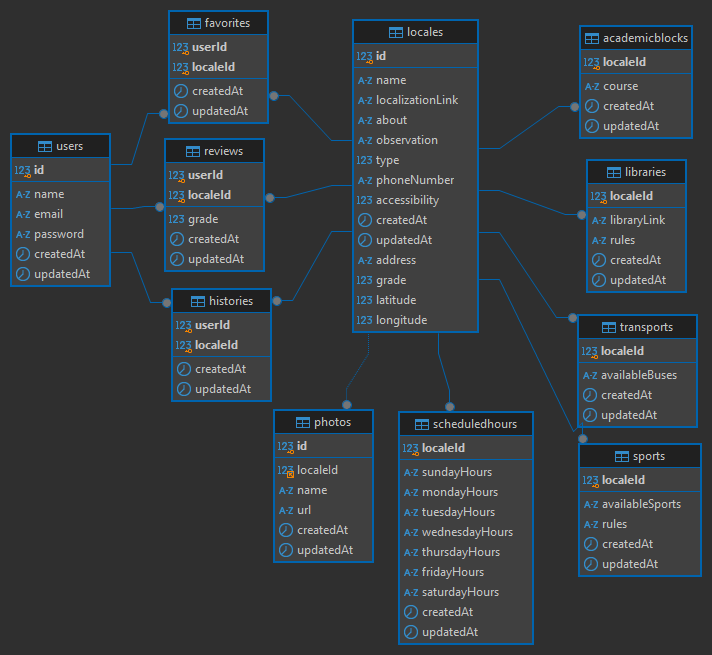
\includegraphics[width=0.7\textwidth]{imagens/encontrenaufms.png}
    \caption{\scriptsize Interface do DBeaver exibindo a estrutura do banco de dados \cite{dbeaver}.}
    \label{fig:descricaoBancoDeDados}
\end{figure}

    Como descrito na Figura 2, o centro da aplicação e do banco de dados são locais. A estrutura do banco foi modelada para permitir uma organização eficiente das informações, com tabelas que representam tanto os locais quanto os atributos e relacionamentos associados:

    \begin{itemize}
        \item \textbf{Locales}: Armazena os dados gerais de cada local, como nome, descrição, e localização.
        \item \textbf{Schedules}: Relacionamento de um para um com a tabela Locales, responsável por armazenar os horários de funcionamento dos locais ao longo da semana.
        \item \textbf{Photos}: Relacionamento de um para muitos com a tabela Locales, onde cada local pode ter diversas fotos associadas.
        \item \textbf{Users}: Armazena os dados do usuário, como nome, email, senha.
        \item \textbf{Histories}: Relacionamento de muitos para muitos com a tabela Locales e a tabela Users, onde cada usuário pode ter um histórico de locais visualizados recentemente.
        \item \textbf{Reviews}: Relacionamento de muitos para muitos com a tabela Locales e a tabela Users, armazena as avaliações de cada usuário feitas aos locais.
        \item \textbf{Favorites}: Relacionamento de muitos para muitos com a tabela Locales e a tabela Users, onde cada usuário pode ter locais favoritos.
        \item \textbf{AcademicBlocks}: Tabela exclusiva para armazenar os nomes dos cursos pertencentes ao respectivo bloco acadêmico.
        \item \textbf{Libraries}: Tabela exclusiva para armazenar as as regras e o link para site externo da biblioteca.
        \item \textbf{Sports}: Tabela exclusiva para armazenar as regras e os esportes disponíveis para serem praticados no centro de esportes.
        \item \textbf{Transportes}: Tabela exlusiva para armazenenar os ônibus que passam no local.
    \end{itemize}

    A tabela ``Locales'' armazena os dados gerais que compõem um determinado local. Sendo que cada local pode possuir horários de funcionamento durante a semana, sendo armazenado na tabela ``Schedules''. Os locais também podem ter fotos, sendo armazenados na tabela ``Photos''.
    
    Os locais foram dividos em tipos específicos para melhor organização dos dados e apresentação ao usuário final, sendo eles: Blocos Acadêmicos, Pontos Turísticos, Bancos, Restaurantes, Serviços de Saúde, Bibliotecas, Centros de Esportes, Transportes, Estacionamentos e Prédios Gerais. Alguns desses tipos posssuem tabelas próprias com informações específicas, como é o caso dos tipos: Blocos Acadêmicos, Bibliotecas, Centros de Esportes e Transportes. 
    
    Além disso, também foi criado uma tabela ``Users'' para armazenar os dados básicos do usuário para cadastro e login do mesmo dentro do sistema. Os usuários possuem 3 relações com a tabela ``Locales'', formando 3 tabelas, sendo elas: ``Histories'', ``Reviews'' e ``Favorites'', que armazenam respectivamente:
    
    \begin{itemize}
        \item O histórico dos 10 últimos locais visualizados recentemente
        \item As avaliações que o usuário fez aos locais 
        \item Os locais favoritos.
    \end{itemize}

    Para a conexão entre o Node.js e o MySQL, foi utilizado o Drizzle que é uma ferramenta de mapeamento de objetos, cujo o foco é a velocidade de entrega de dados entre as duas ferramentas. 

\subsection{Testes e Execução}

    O aplicativo Encontre na UFMS foi testado em diversos dispositivos Android, a fim de garantir a compatibilidade e o bom funcionamento em diferentes tamanhos de tela e versões do sistema operacional. Foi utilizado o emulador do Android Studio para testar o aplicativo no Pixel 6a na API 33 do Android mas foi principalmente testado em dispositivos físicos, como o Galaxy S21 fe e Xiomi Note 8 Pro, pela facilidade de uso e para poder verificar a usabilidade real do aplicativo em todo momento.

\subsubsection{Diagrama de Navegação}

    A Figura 3 ilustra o diagrama de navegação do aplicativo Encontre na UFMS:

    \begin{figure}[h]
        \centering
        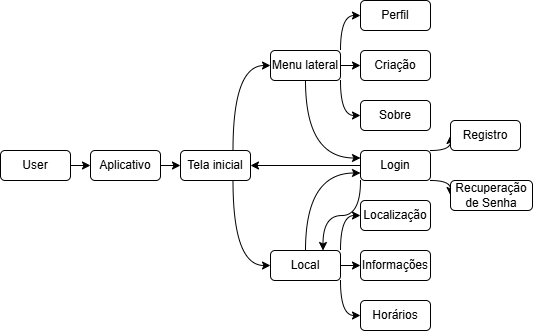
\includegraphics[width=120mm,height=70mm]{imagens/navegacao.png}
        \caption{\scriptsize Diagrama de Navegação}
        \label{fig:diagrama-navegacao}
    \end{figure}

    O diagrama de navegação do aplicativo apresentado acima demonstra os fluxos básicos de navegação que o usuário pode experenciar
    durante o uso do mesmo, vale destacar que algumas telas como Perfil e Criação só são acessíveis caso o usuário esteja logado.

    \FloatBarrier

\subsubsection{Tela 1: Listagem de Locais}

    A tela de listagem de locais é a tela inicial do aplicativo, a primeira e principal tela apresentada para o usuário. Nela, o usuário pode visualizar todos os locais cadastrados no aplicativo, podendo filtrar os locais por categoria e buscar locais através de um campo de pesquisa por texto. 
    
    Cada local é representado por um segmento contendo a foto, o nome, o endereço, a categoria, se o local está provavelmente fechado naquele horário e um indicador que mostra se o local está marcado como favorito ou não. Cada segmento é clicável, redirecionando o usuário para a tela de detalhes do local. O usuário pode também clicar no indicador de favorito para marcar ou desmarcar o local como favorito caso ele esteja logado, caso não esteja o usuário é redirecionando para a tela de Login que será abordada mais a frente. A listagem de locais é paginada, exibindo 10 locais por vez, uma nova requisição é feita toda vez que o usuário chega ao final da lista, carregando a próxima página, se houver.

    Na parte superior da tela há uma seção com um botão, que abre o menu lateral, e um campo de texto para pesquisa. Logo abaixo há um filtro de categorias, uma série de botões que podem ser arrastados horizontalmente, permitindo que o usuário filtre os locais por uma ou mais categorias, de acordo com suas necessidades. Na busca por texto foi aplicado um \textit{debounce} de 1s para evitar que a busca seja feita a cada caractere digitado, o que poderia causar um consumo excessivo de recursos da API. A Figura 4 mostra a tela de listagem de locais.

    \begin{figure}[h]
        \centering
        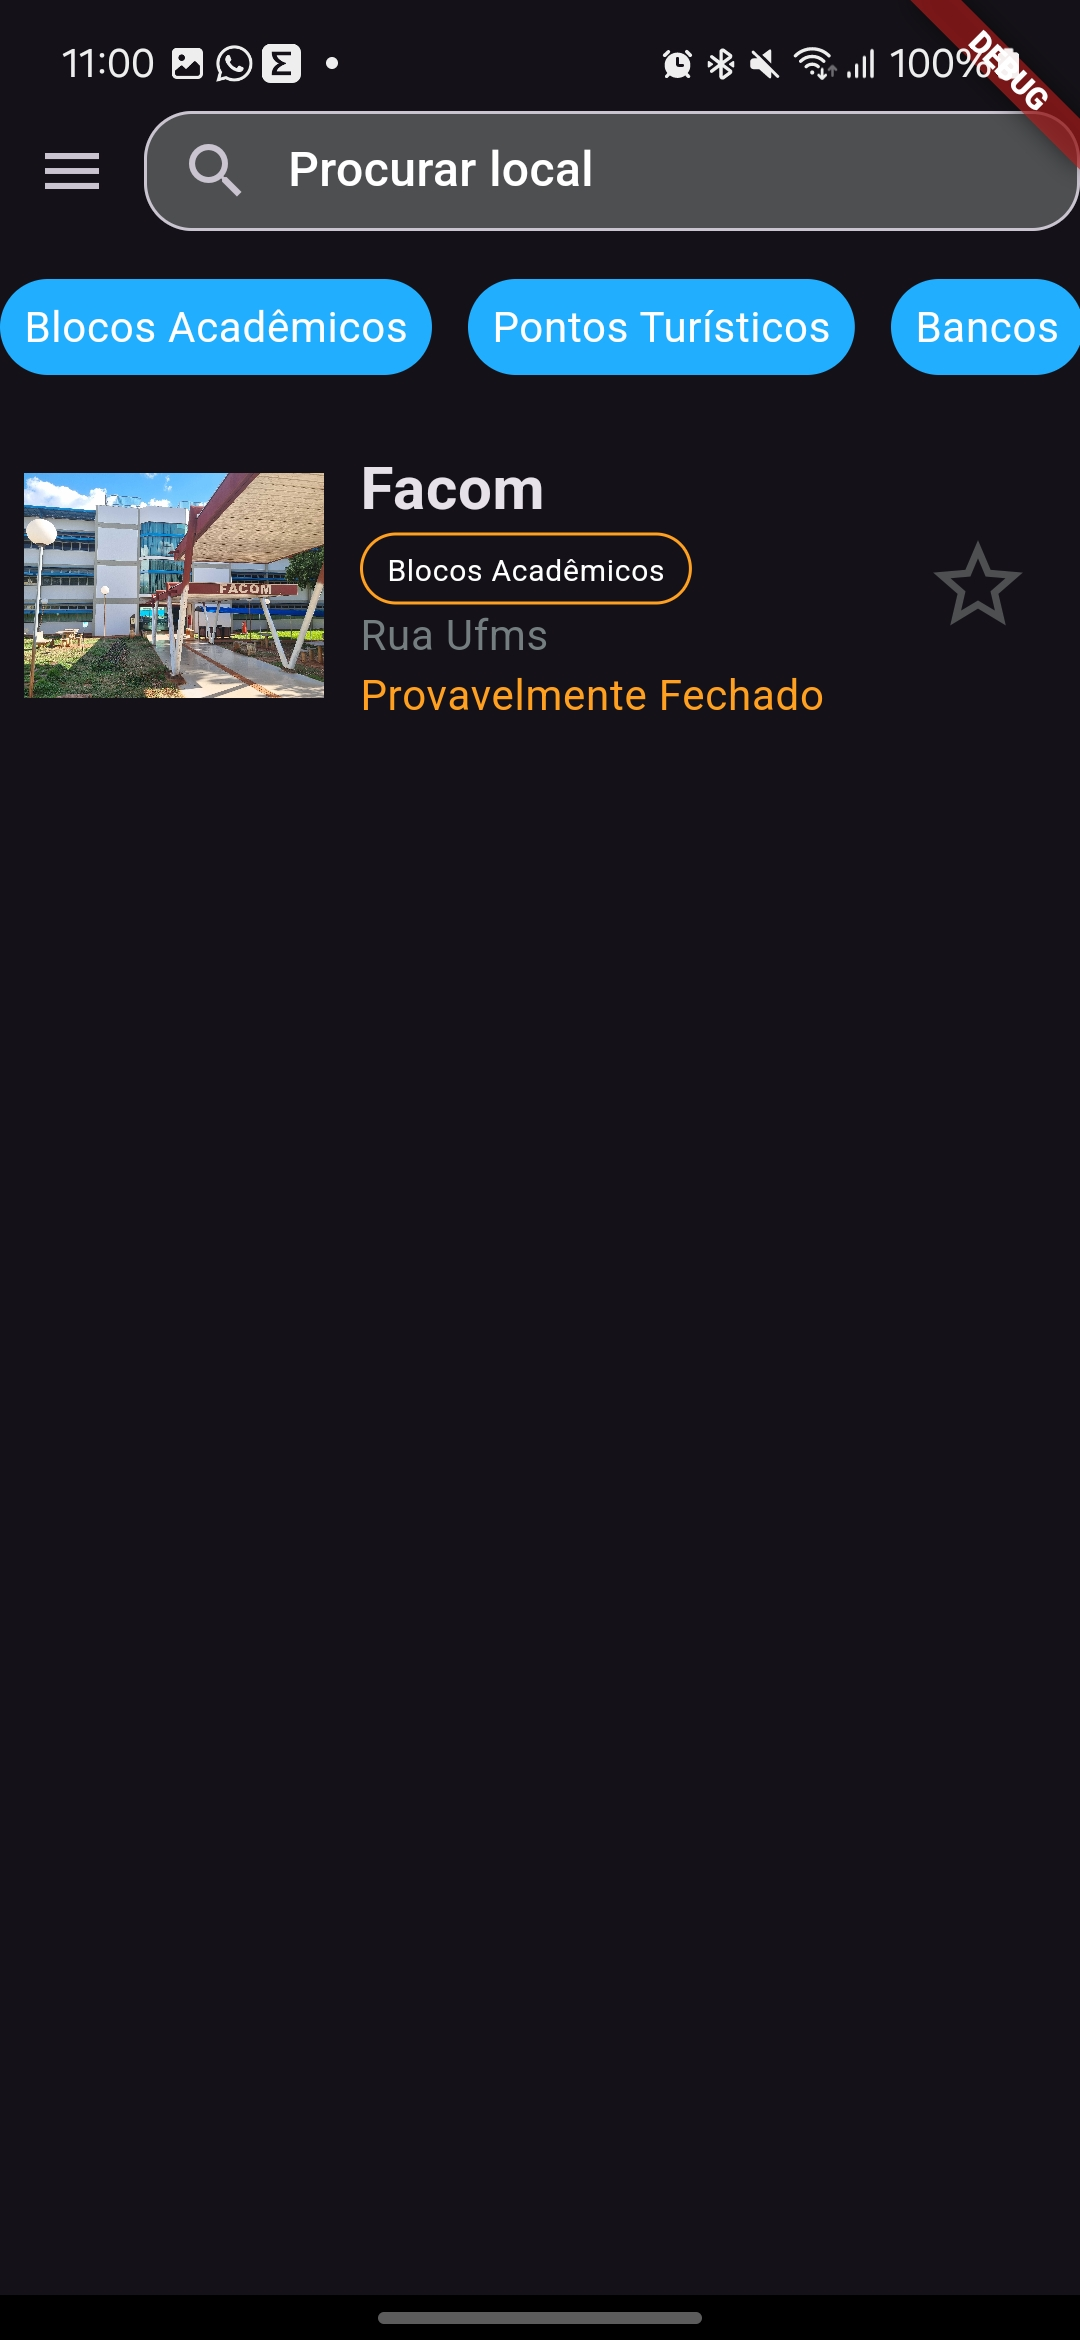
\includegraphics[width=44mm,height=80mm]{imagens/inicial.jpg}
        \caption{\scriptsize Tela 1: Listagem de Locais}
        \label{fig:tela1}
    \end{figure}

    \FloatBarrier

\subsubsection{Tela 2: Local}

    A tela de local apresenta todos os detalhes do local que foi selecionado pelo usuário. Nela, o usuário pode visualizar uma ou mais fotos do local, o nome, um indicador que é mostrado caso o local tenha opções de acessibilidade e a avaliação média do local, que é a média das avaliações por outros usuários. Além disso existem 3 abas que o usuário pode navegar sem sair da tela. A aba de localização é a aba inicial e mostra o endereço do local, um mapa com a localização do local indicada e uma seção para o usuário dar sua própria avaliação do local, caso esteja logado. A aba de informações exibe alguns detalhes do local como observações e telefone de contato. Por fim, a aba de Horários exibe os horários de funcionamento do local, caso estejam cadastrados. A Figura 5 mostra a tela de local com a aba de localização, já a Figura 6 apresenta as demais abas.

    \begin{figure}[h]
        \centering
        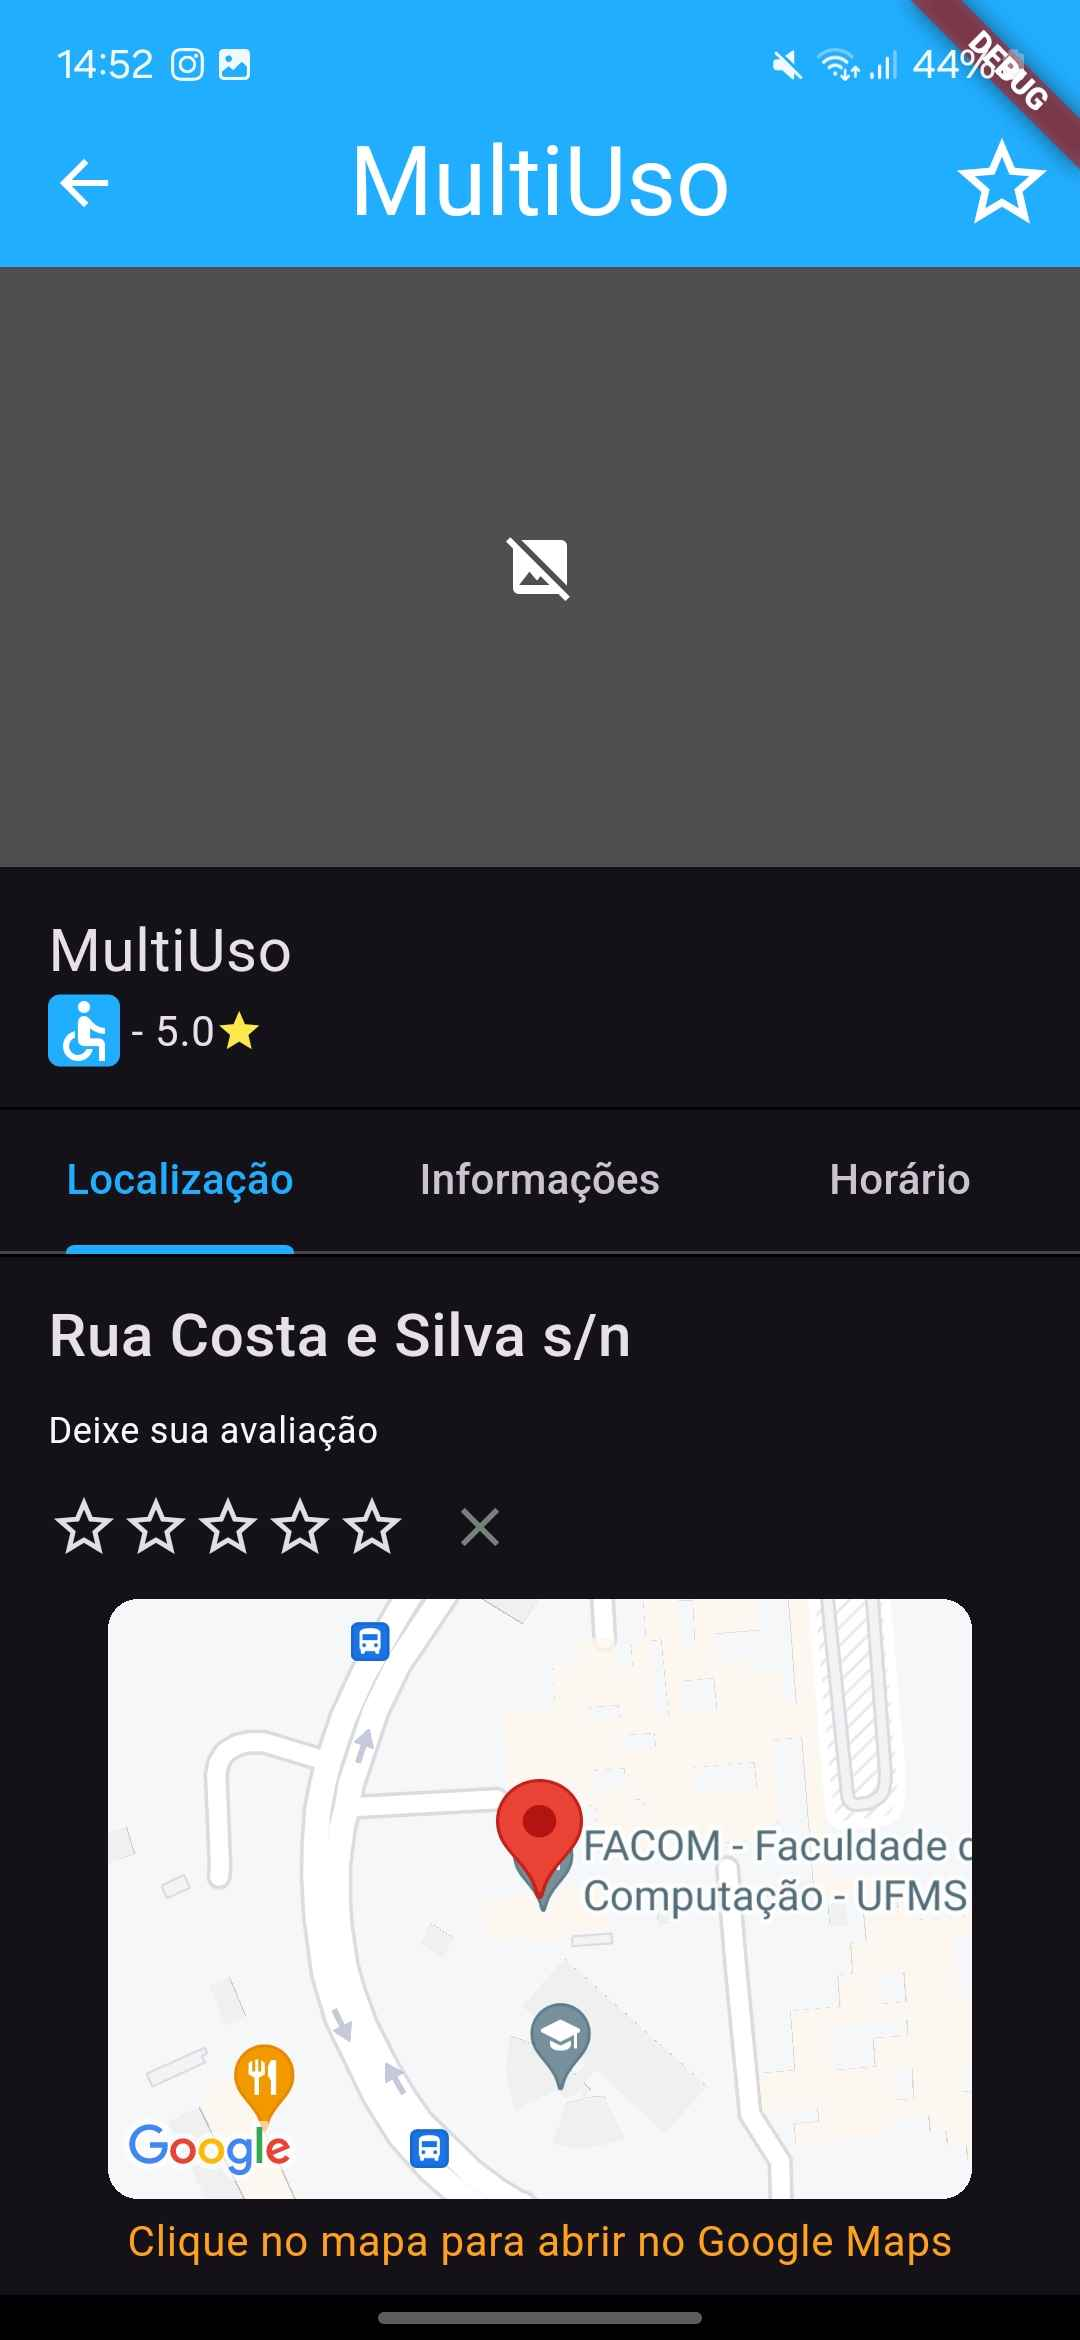
\includegraphics[width=44mm,height=80mm]{imagens/local.jpg}
        \caption{\scriptsize Tela 2: Local}
        \label{fig:tela2}
    \end{figure}

    \begin{figure}
        \centering
        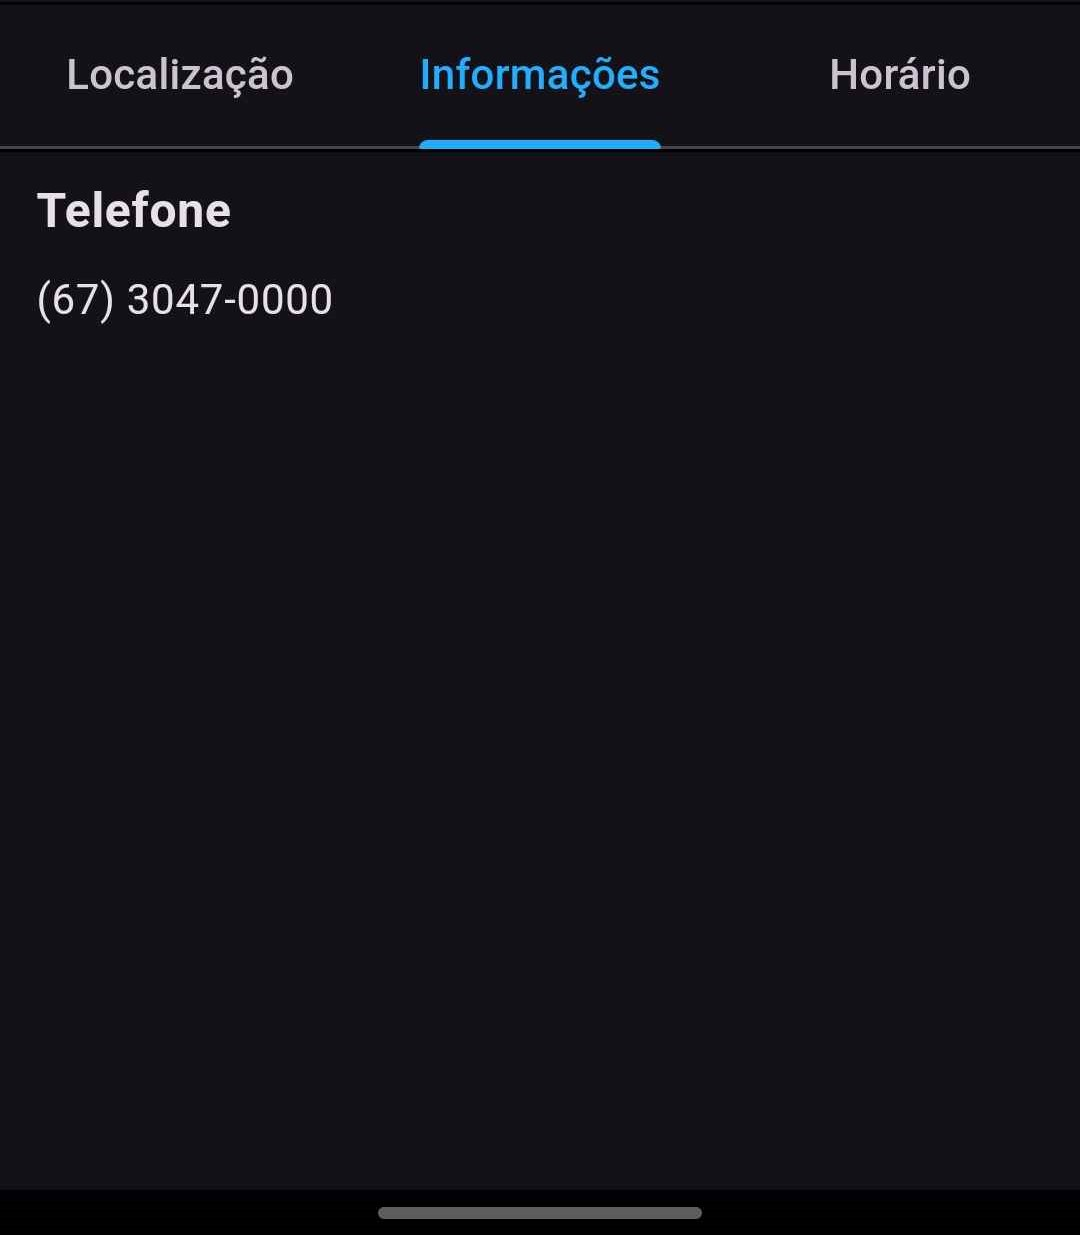
\includegraphics[width=44mm,height=48mm]{imagens/info.jpg}
        \hspace{10mm}
        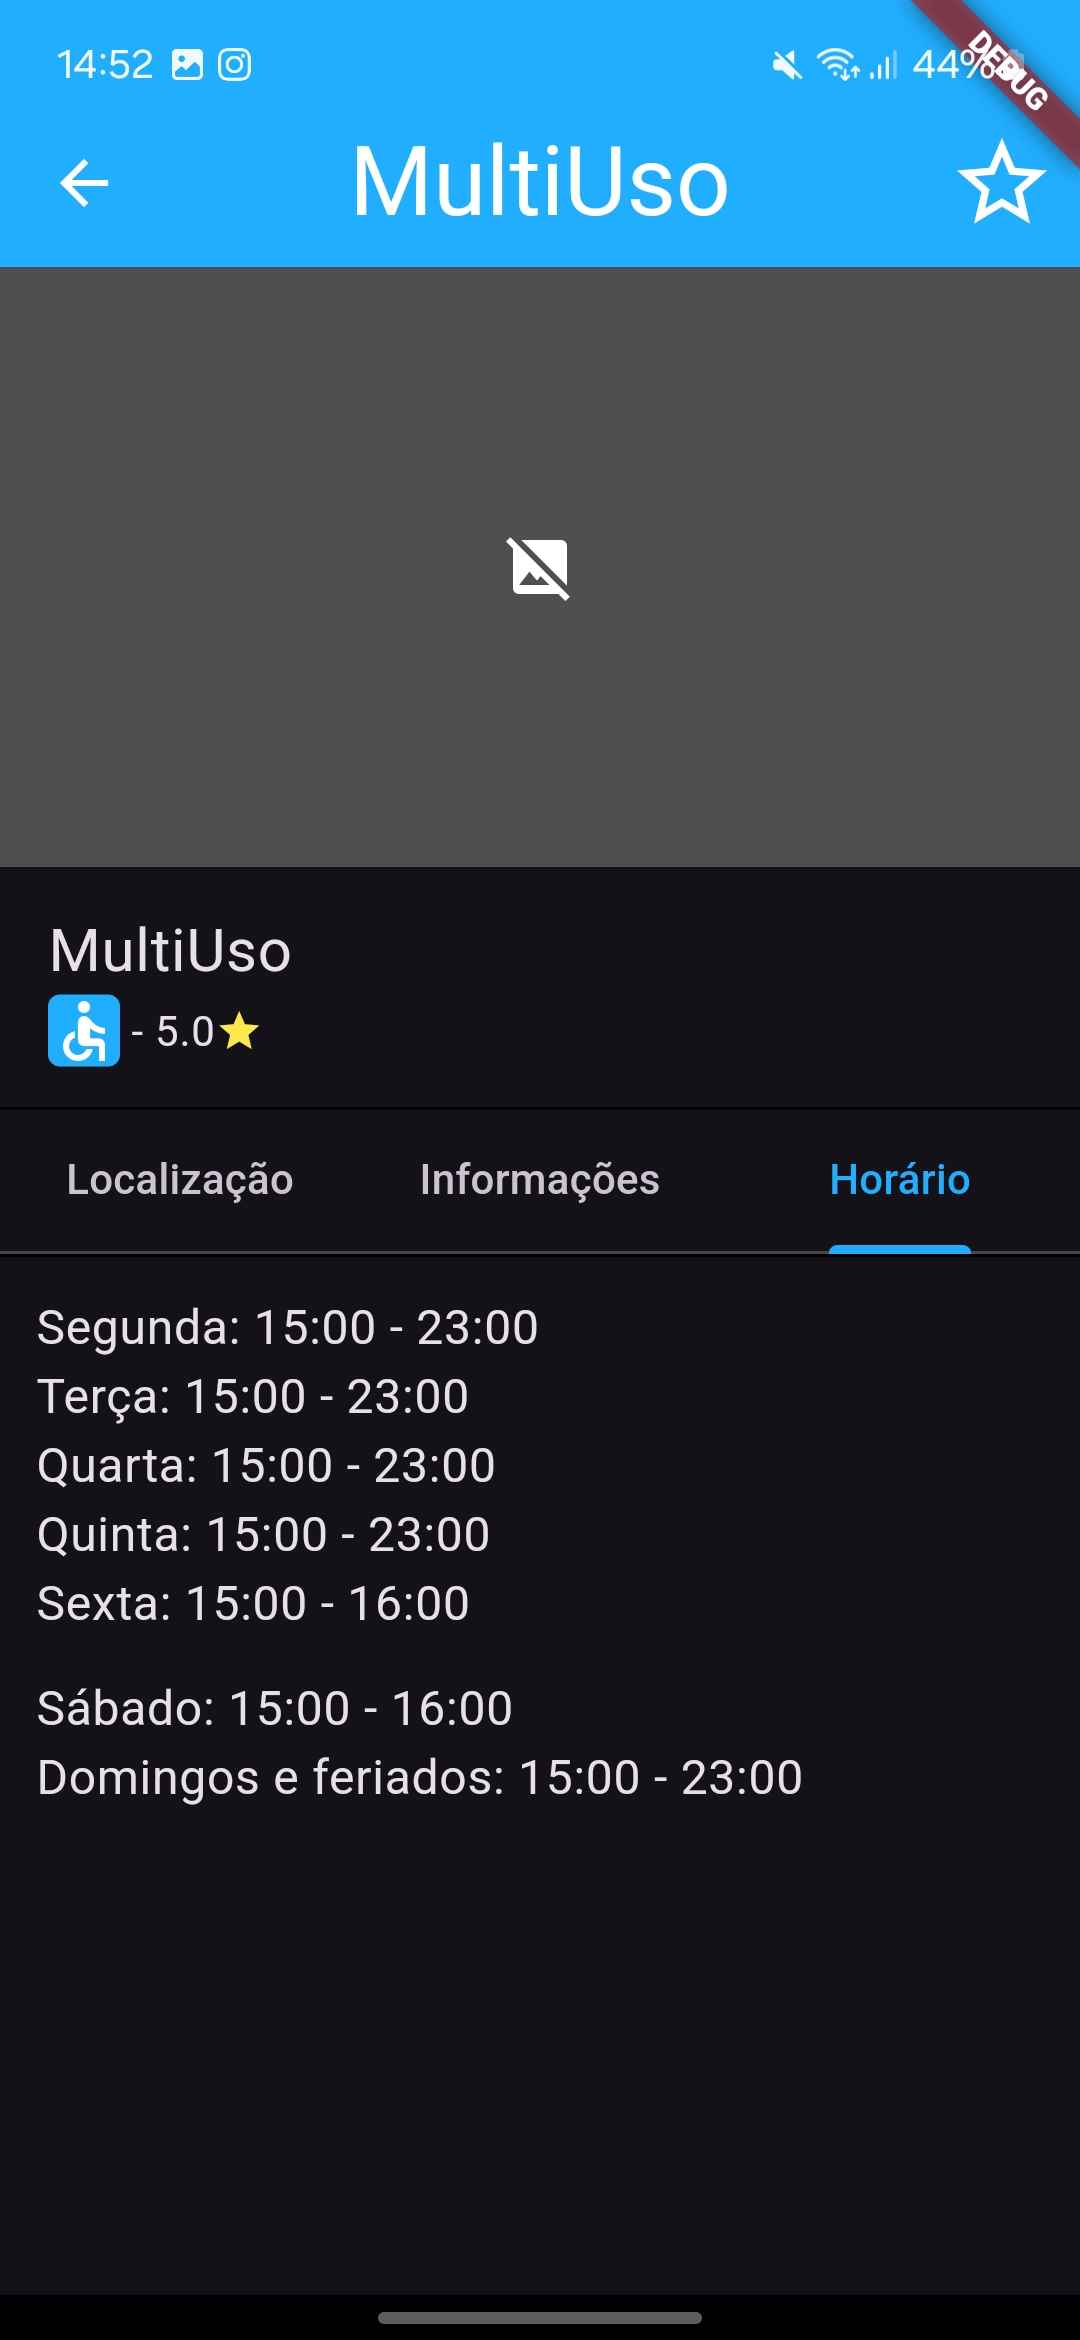
\includegraphics[width=44mm,height=48mm]{imagens/horario.jpg}
        \caption{\scriptsize Abas: Informações e Horários}
        \label{fig:tela2-abas}
    \end{figure}

    \FloatBarrier

\subsubsection{Tela 3: Menu Lateral}

    O menu lateral é acessível através de um botão na parte superior da tela de listagem de locais. Ele é composto por uma série de botões que redirecionam o usuário para diferentes telas do aplicativo. O menu lateral é uma forma de organizar as funcionalidades do aplicativo de forma intuitiva e acessível, permitindo que o usuário navegue facilmente entre as diferentes telas do aplicativo.

    Essa tela muda de acordo com o estado de autenticação do usuário, caso ele esteja logado, aparecerá o nome do usuário logo abaixo o nome do aplicativo e os botões de Perfil e Criação assim como um botão de Sair, caso contrário, todas essas informações são omitidas e apenas o botão de Sobre é exibido, e no lugar do botão de Sair é exibido o botão de Login. Abaixo as duas figuras exemplificam ambos os estados. A Figura 7 mostra o menu lateral tanto no estado logado quanto no estado deslogado.

    \begin{figure}[h]
        \centering
        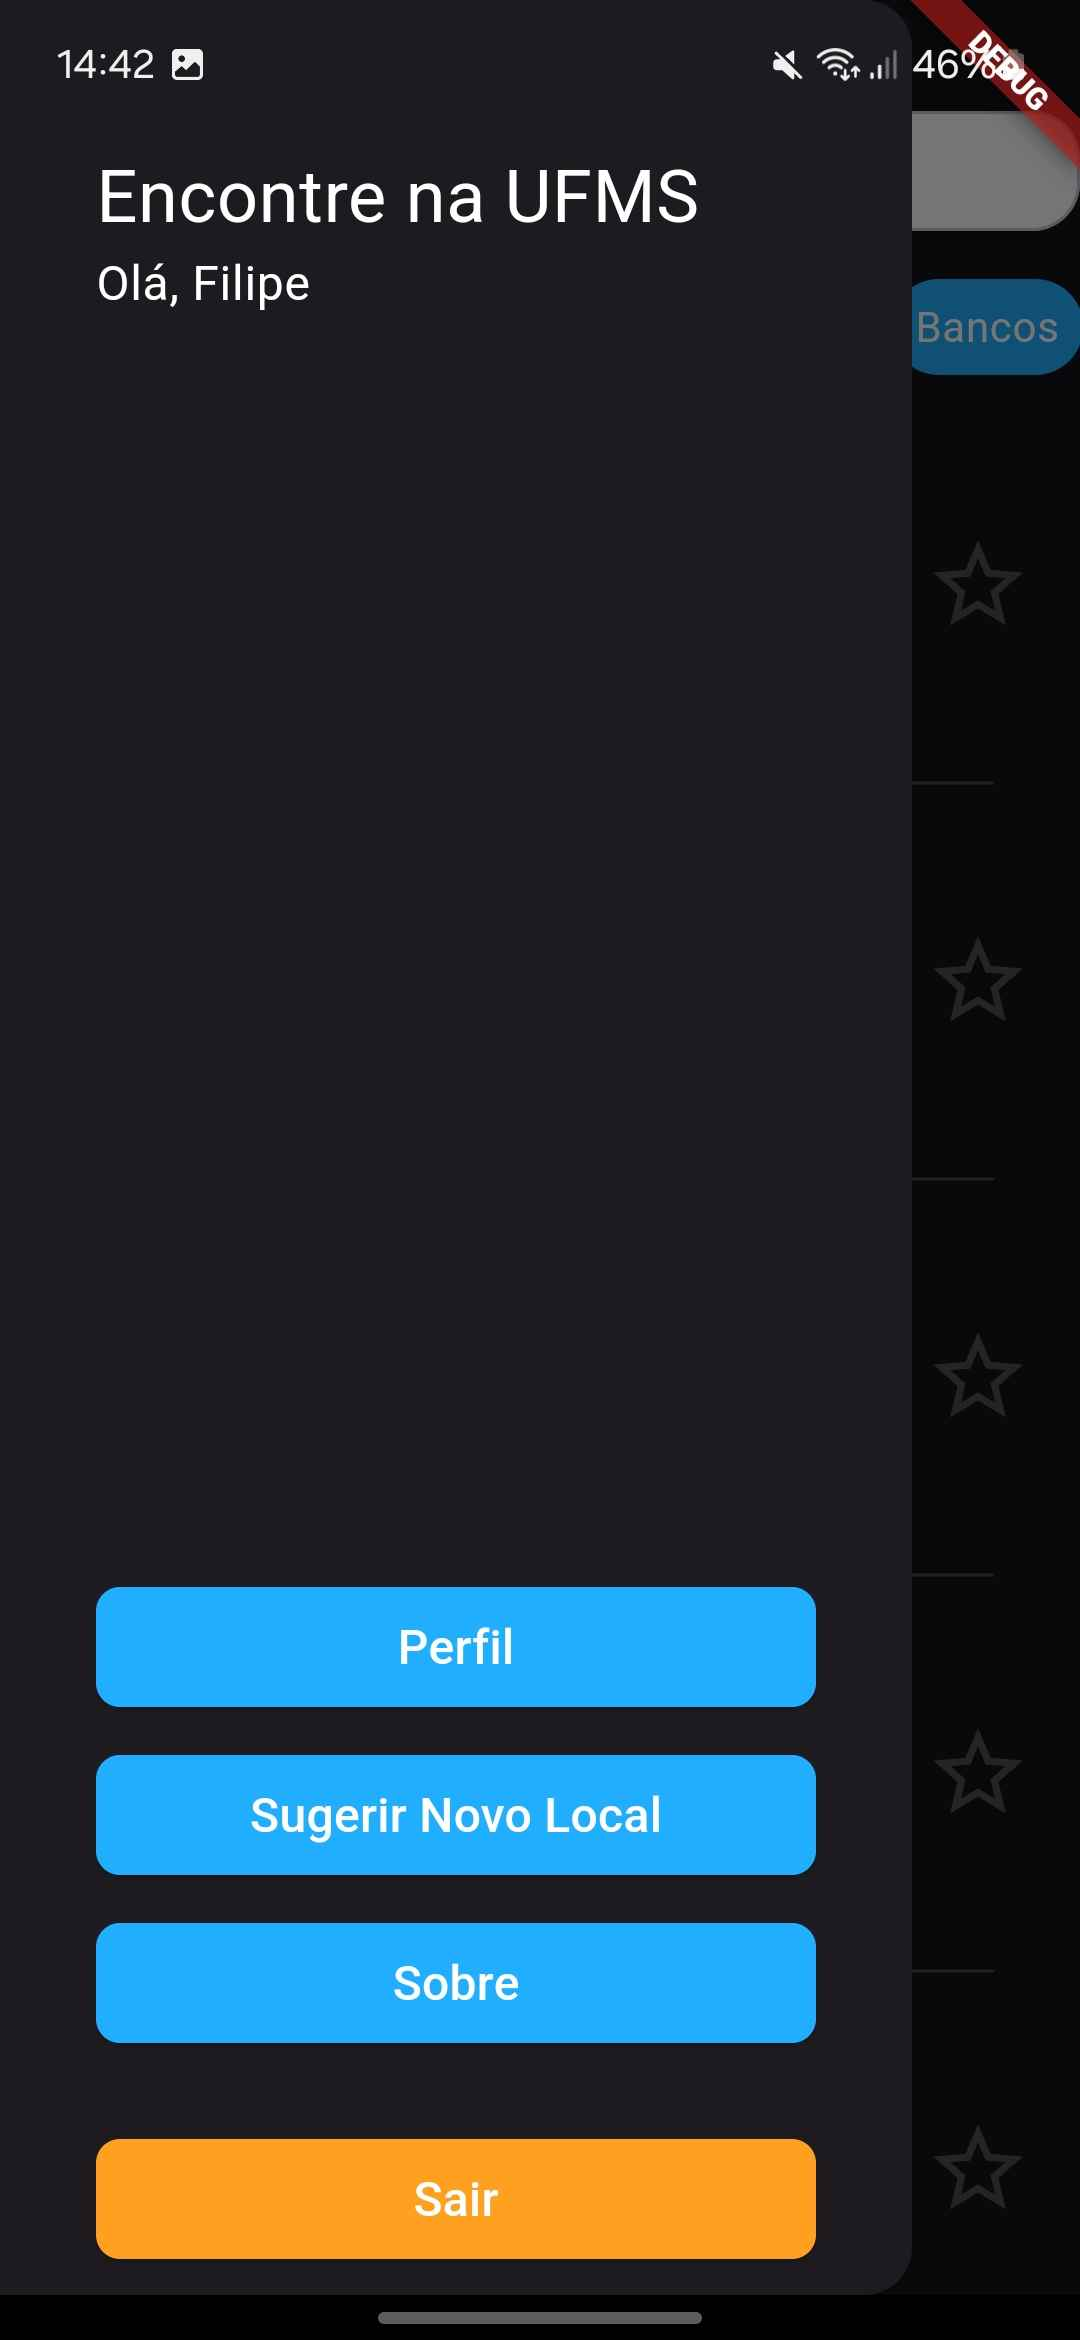
\includegraphics[width=44mm,height=80mm]{imagens/menu-lateral-logado.jpg}
        \hspace{10mm}
        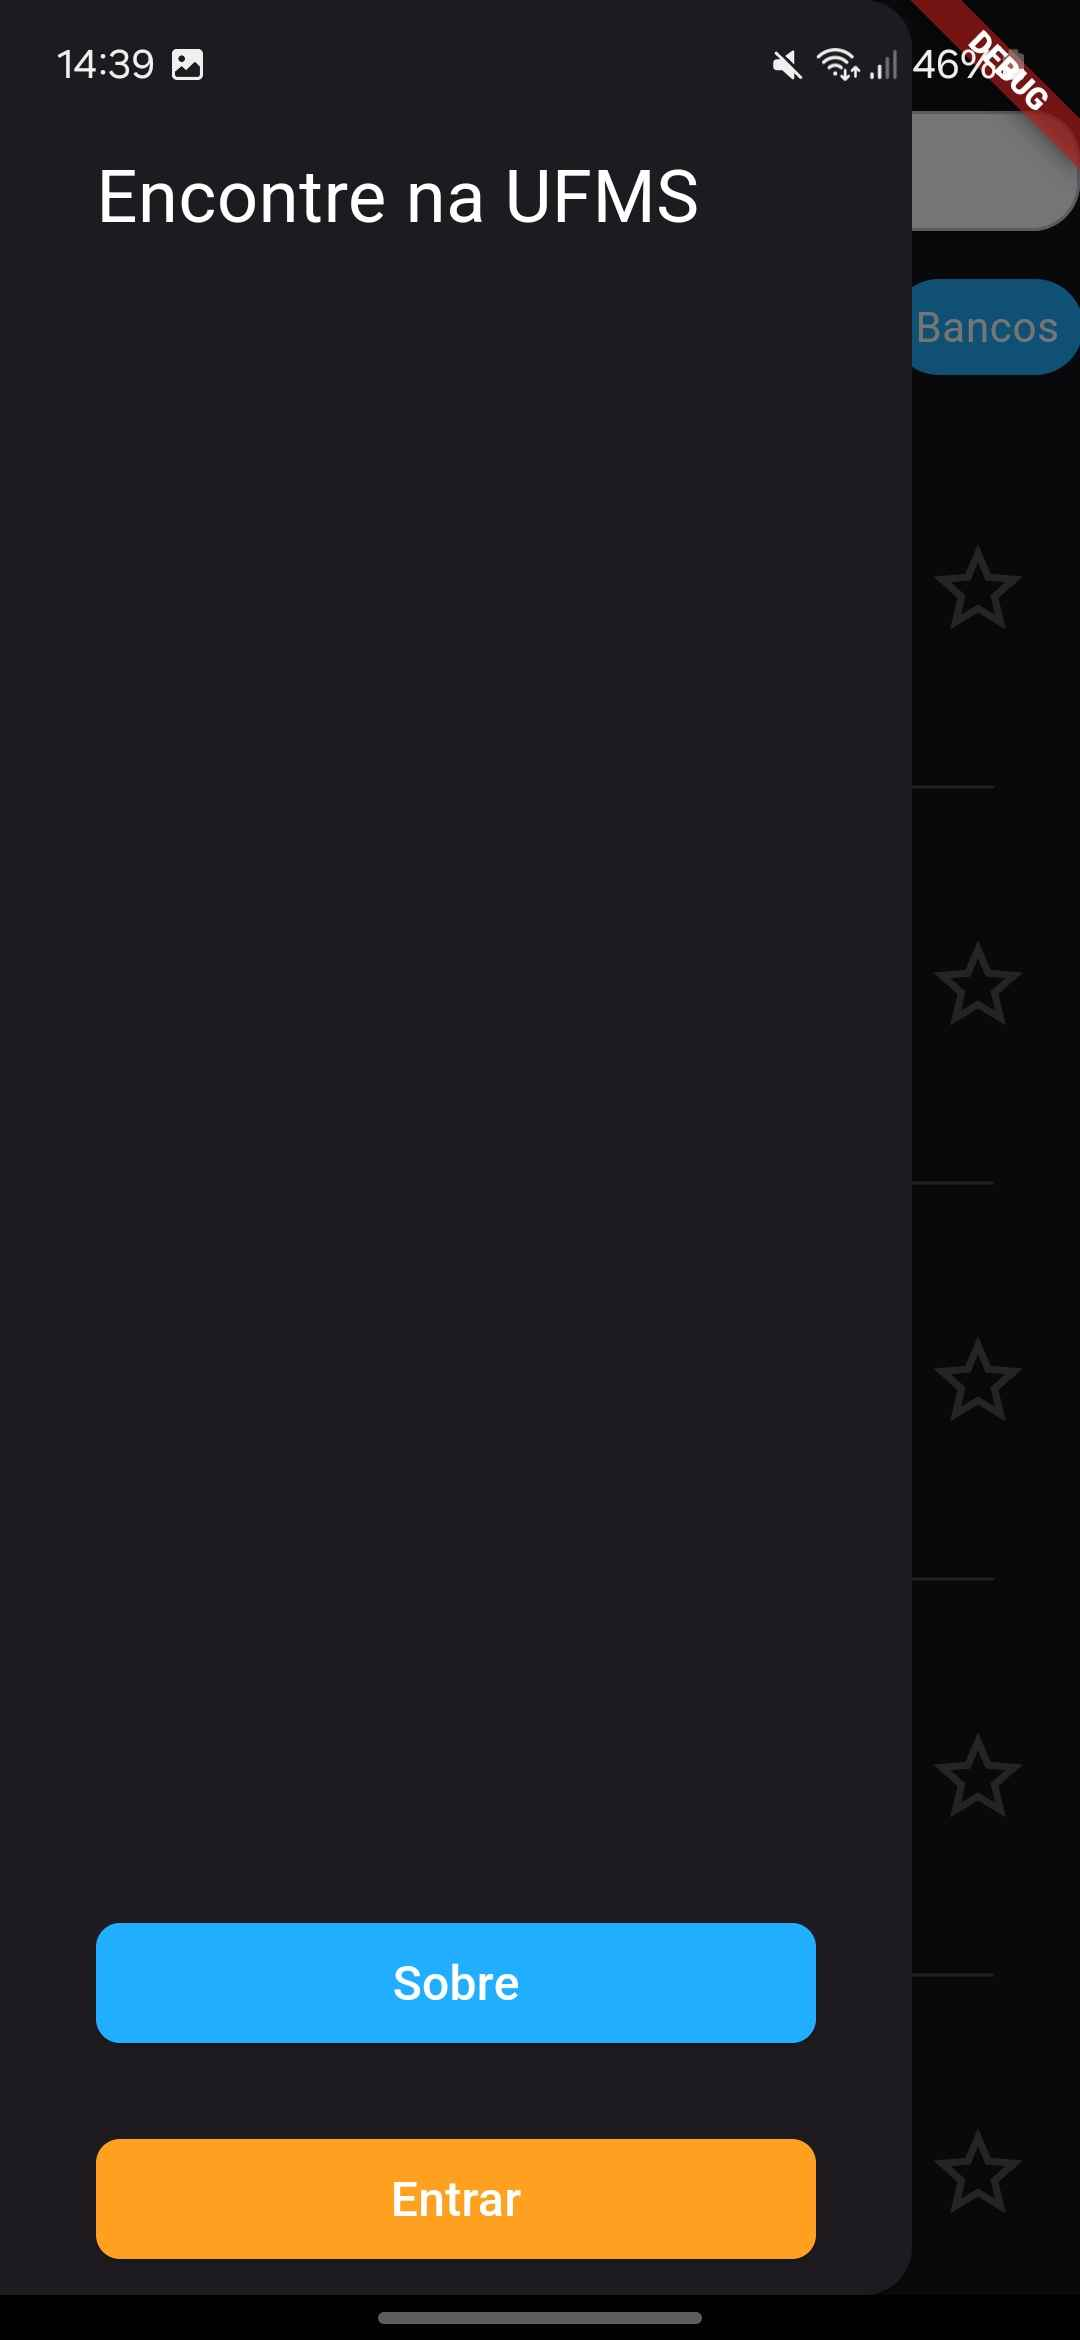
\includegraphics[width=44mm,height=80mm]{imagens/menu-lateral-logout.jpg}
        \caption{\scriptsize Tela 2: Menu Lateral (Logado e Deslogado)}
        \label{fig:tela2-logado}
    \end{figure}

    \FloatBarrier

\subsubsection{Tela 4: Perfil}

    A tela de perfil exibe as informações do usuário logado, nome e e-mail. Além disso, a tela também permite que o usuário edite seu nome e altere sua senha. A tela de perfil é uma forma de o usuário gerenciar suas informações pessoais e garantir que seus dados estejam sempre atualizados. A Figura 8 mostra a tela de perfil.

    \begin{figure}[h]
        \centering
        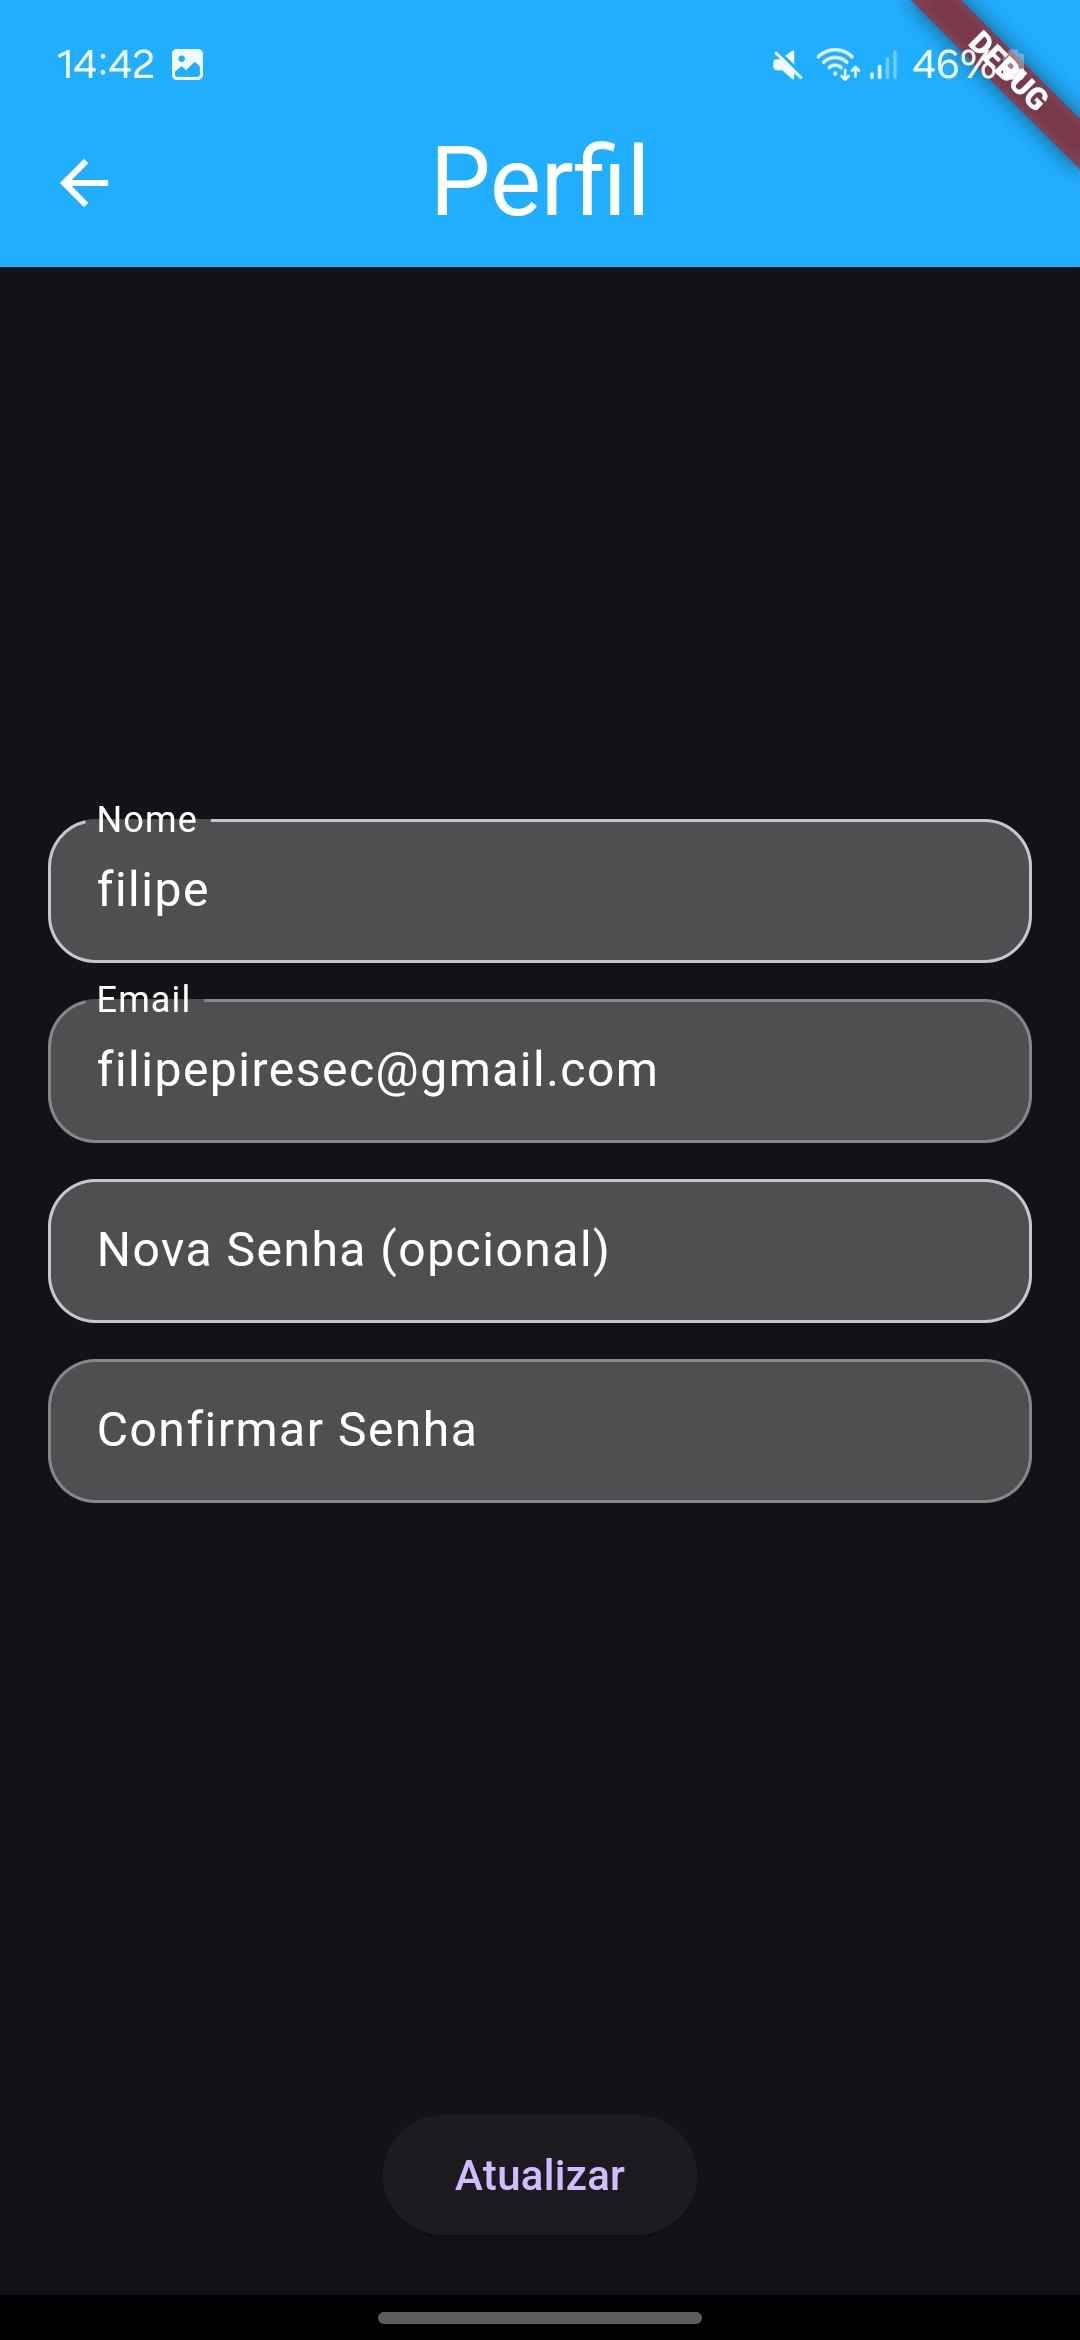
\includegraphics[width=44mm,height=80mm]{imagens/perfil.jpg}
        \caption{\scriptsize Tela 4: Perfil}
        \label{fig:tela4}
    \end{figure}

    \FloatBarrier

\subsubsection{Tela 5: Criação}

    A tela de criação possibilita que os usuários preencham uma série de informações sobre o local que desejam cadastrar, como nome, endereço, categoria, horários de funcionamento, telefone de contato, observações e fotos, e enviem para uma avaliação. A tela de criação é uma forma de os usuários contribuírem com o aplicativo, adicionando novos locais e enriquecendo a base de dados do sistema. A Figura 9 mostra as telas de criação.

    \begin{figure}[h]
        \centering
        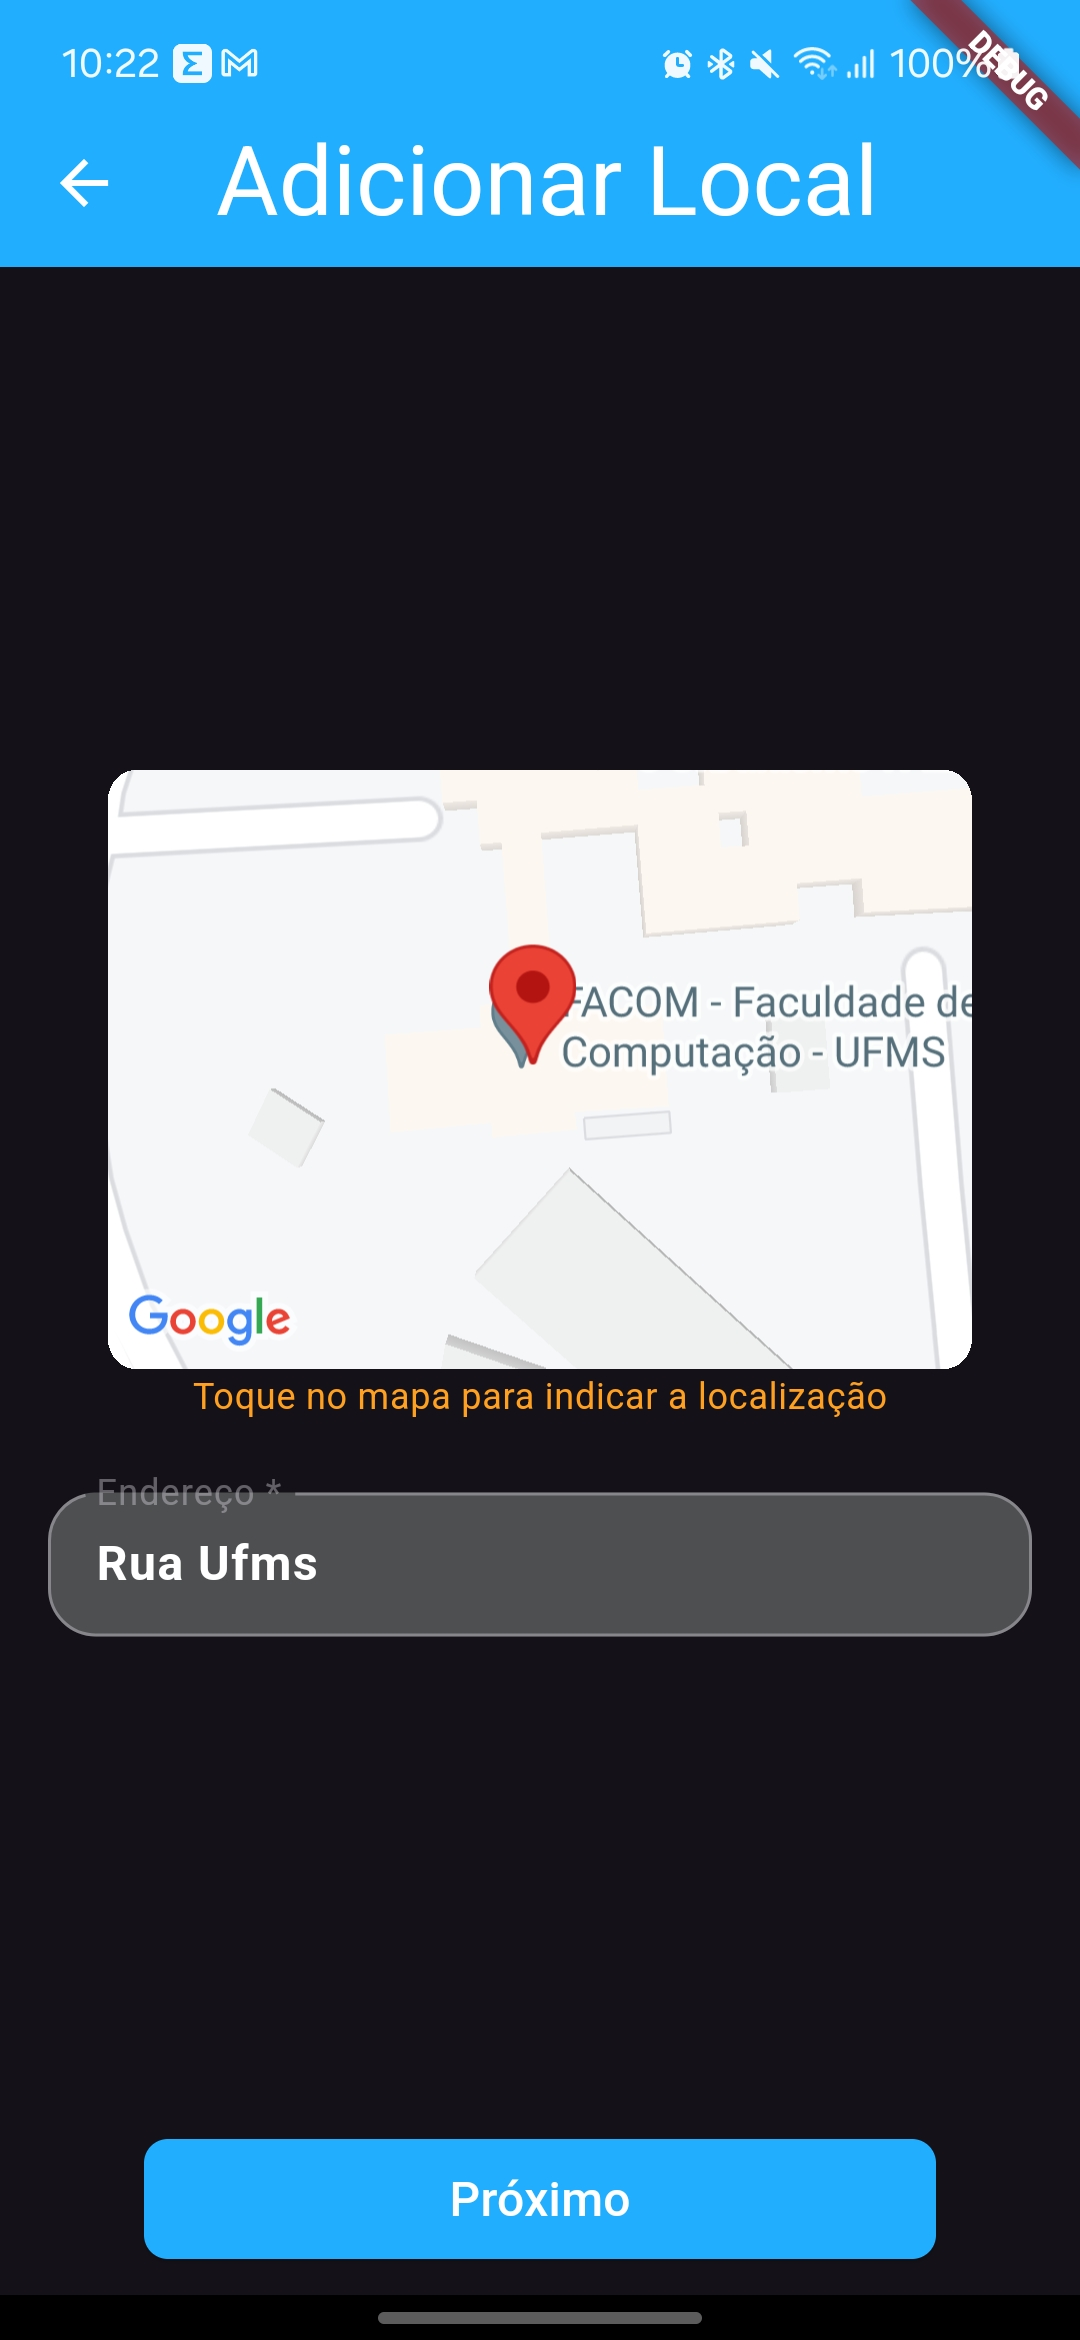
\includegraphics[width=44mm,height=80mm]{imagens/criacao.jpg}
        \hspace{10mm}
        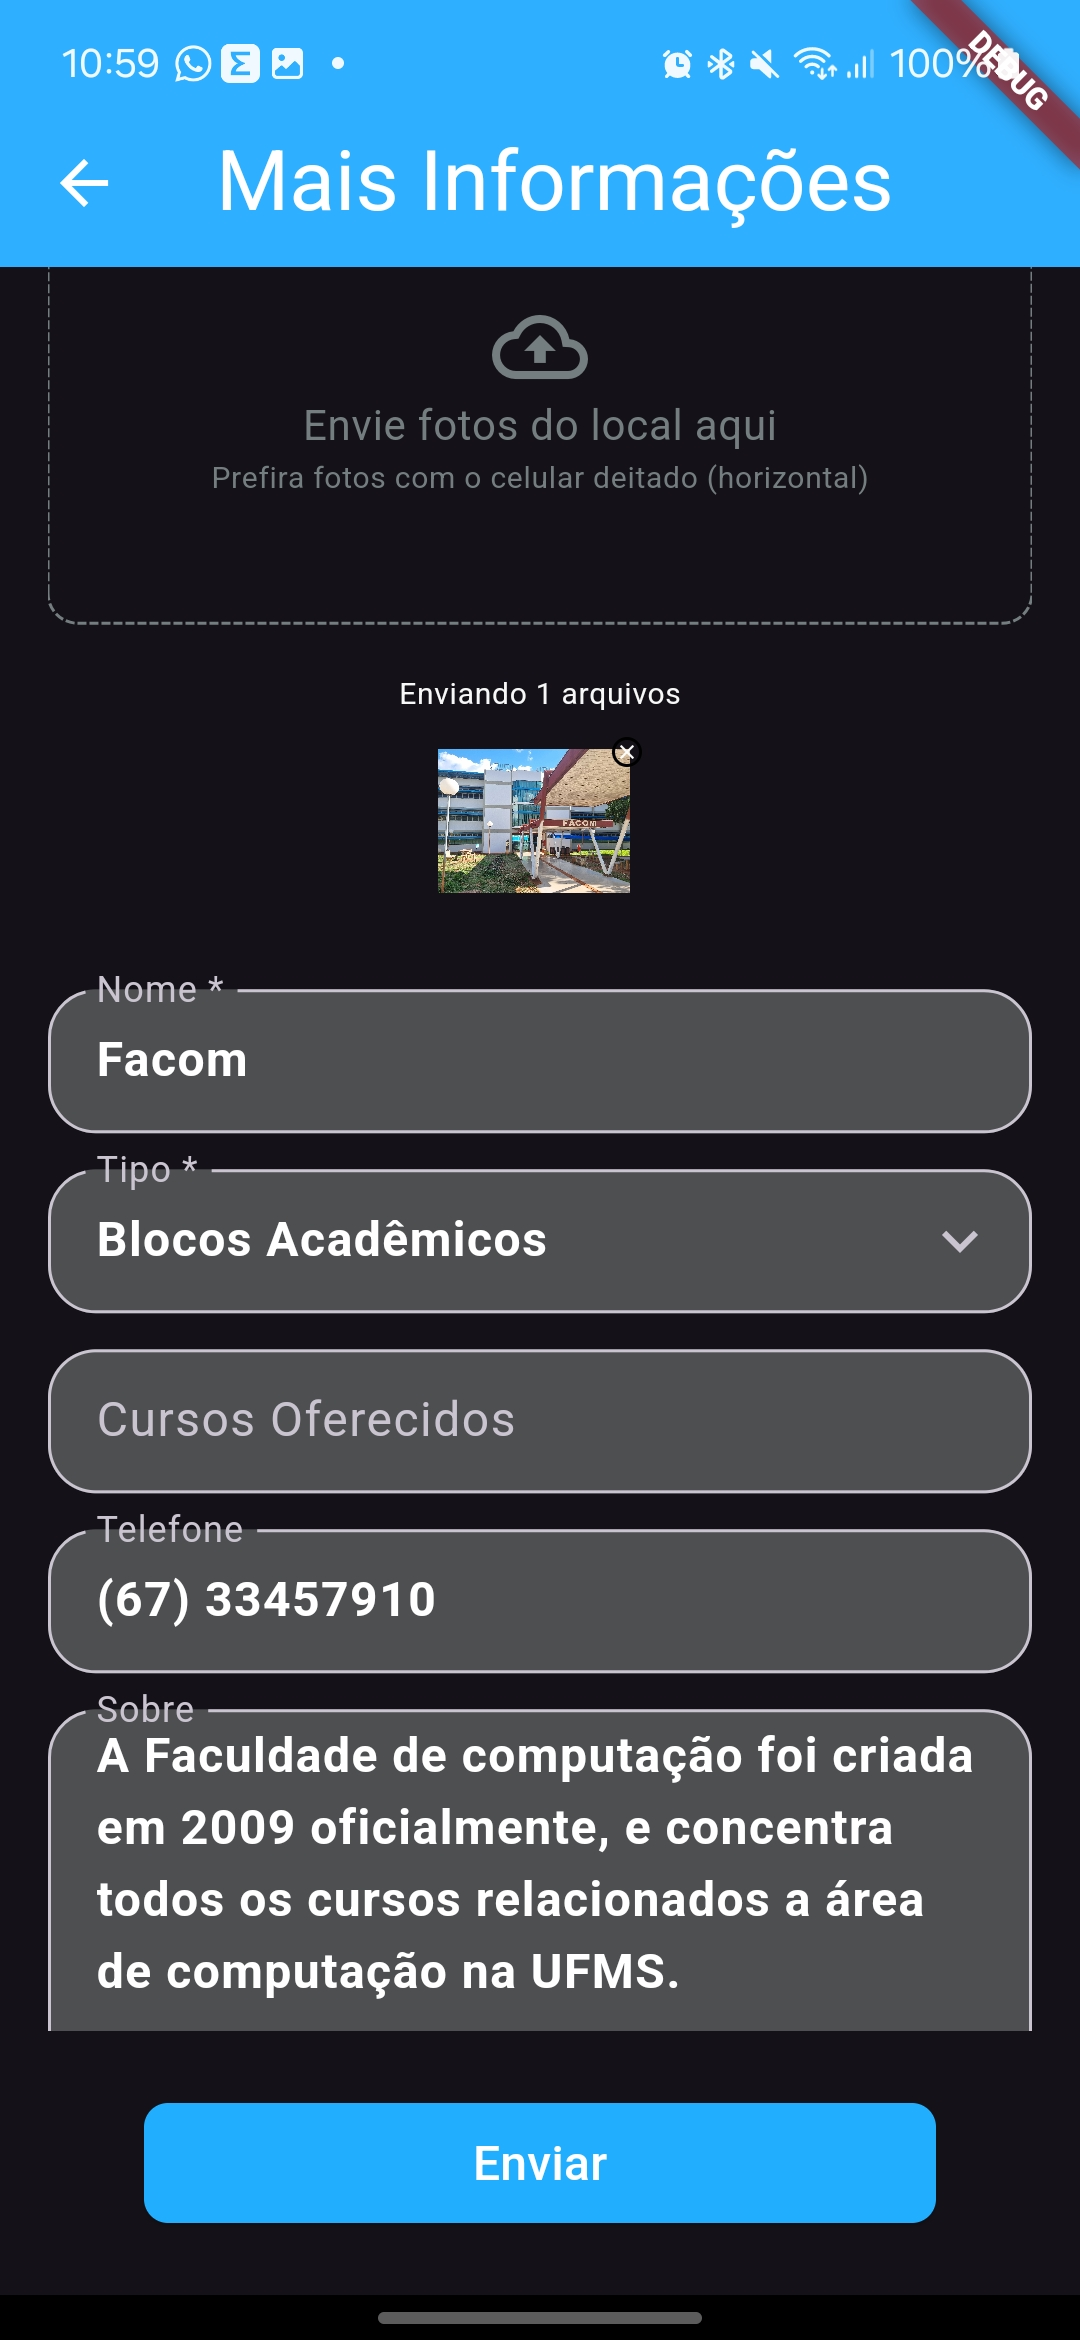
\includegraphics[width=44mm,height=80mm]{imagens/criacao2.jpg}
        \caption{\scriptsize Tela 5: Criação}
        \label{fig:tela5}
    \end{figure}

    \FloatBarrier

\subsubsection{Tela 6: Sobre}

    A tela de sobre exibe informações sobre o aplicativo, como a versão, os desenvolvedores e o código fonte. A tela de sobre é uma forma de os usuários conhecerem mais sobre o aplicativo e os desenvolvedores por trás dele. A Figura 10 mostra a tela de sobre.

    \begin{figure}[h]
        \centering
        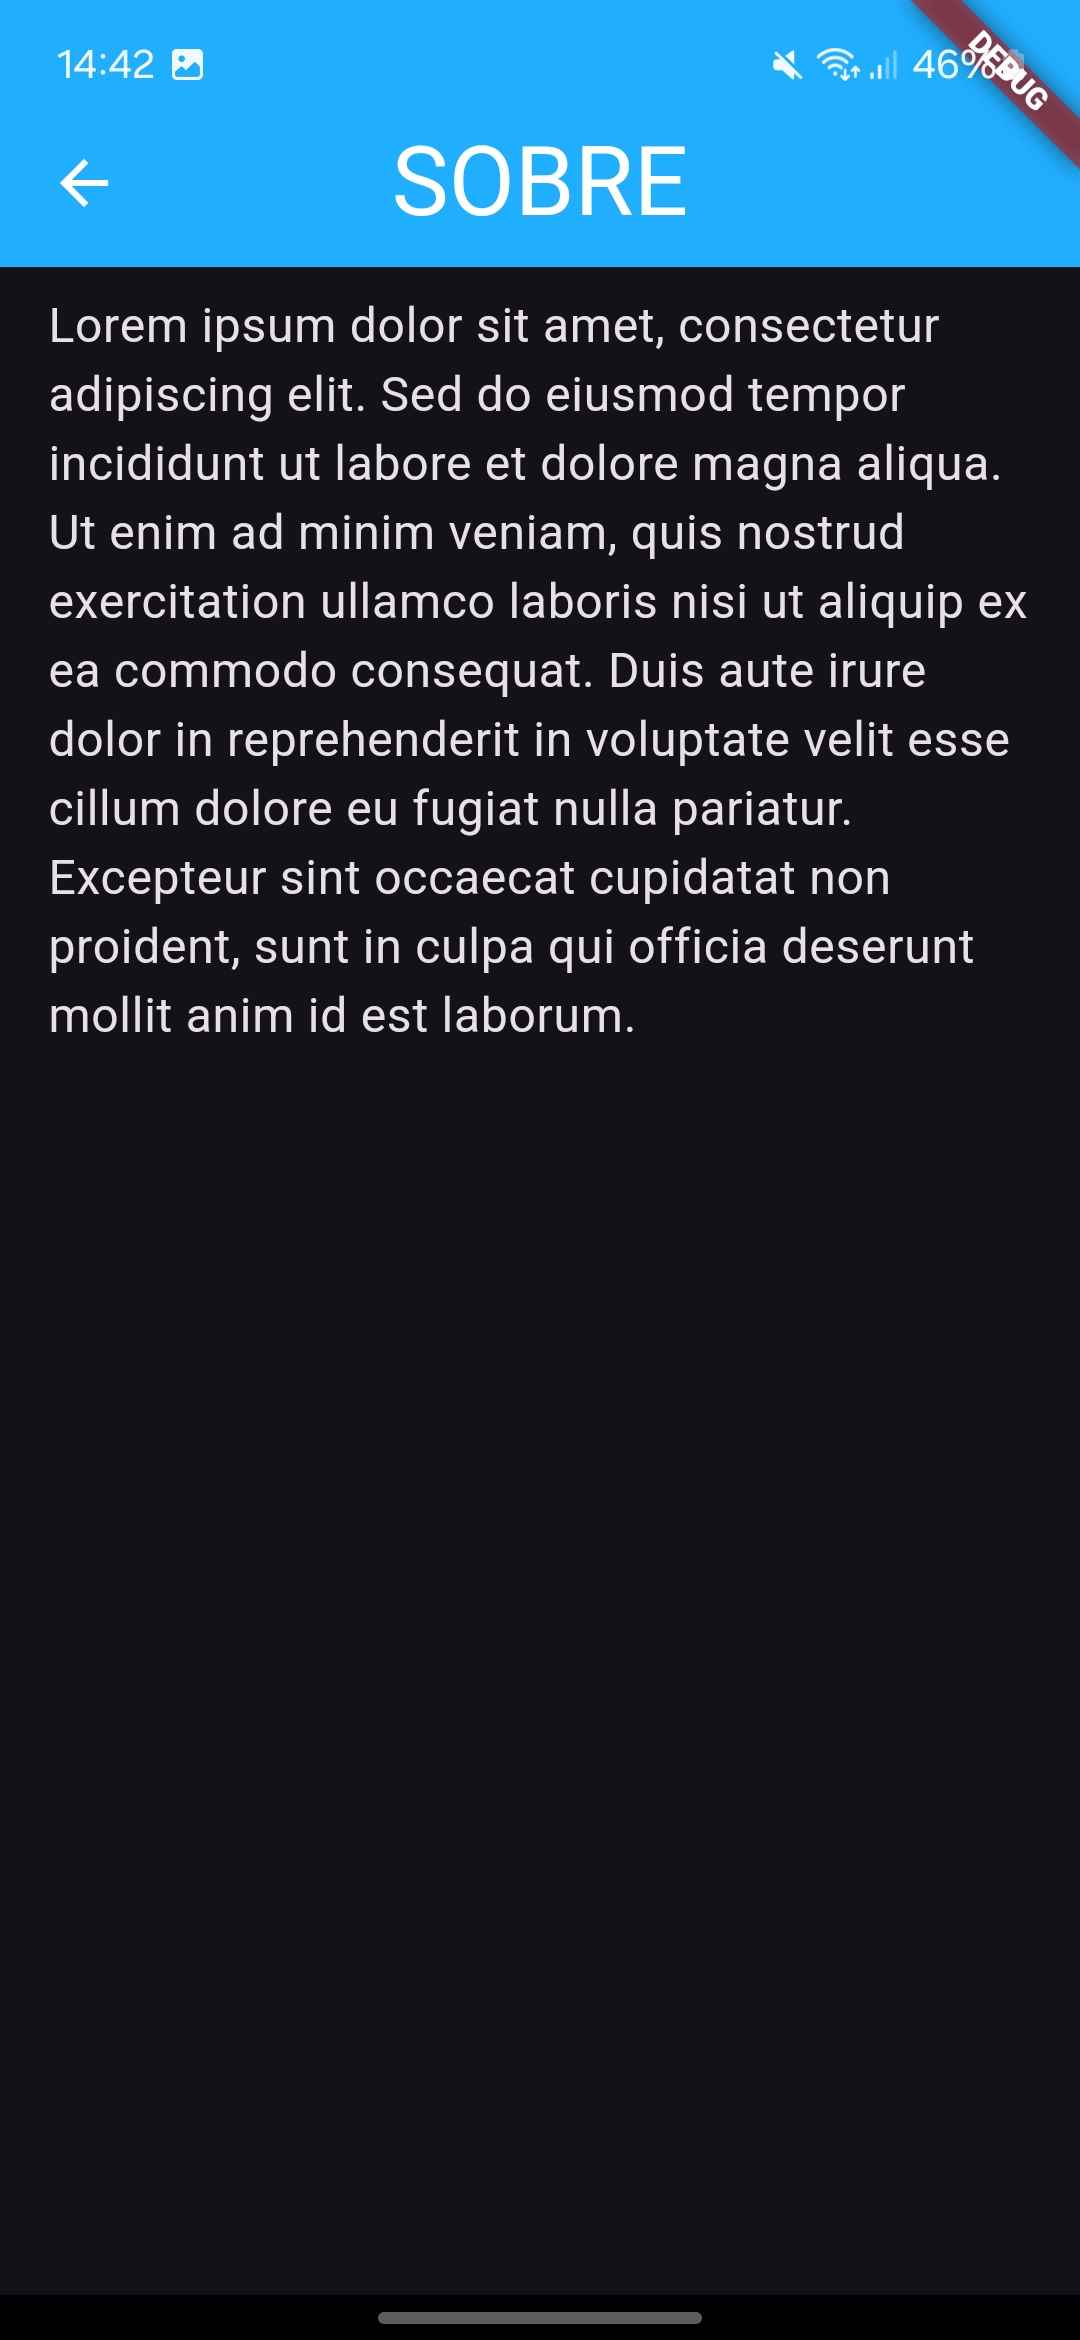
\includegraphics[width=44mm,height=80mm]{imagens/sobre.jpg}
        \caption{\scriptsize Tela 6: Sobre}
        \label{fig:tela6}
    \end{figure}

    \FloatBarrier

\subsubsection{Tela 7: Login}

    A tela de login pode ser alcançada através de 2 fluxos, o primeiro é através do botão de Login na tela de Menu Lateral e o segundo é quando o usuário tentar marcar um local como favorito sem estar logado. A tela de login é composta por um campo de e-mail e um campo de senha, além de botões para iniciar o processo de registro de uma nova conta ou para recuperar a senha, caso o usuário tenha esquecido. A Figura 11 mostra a tela de login e de cadastro.

    \begin{figure}[h]
        \centering
        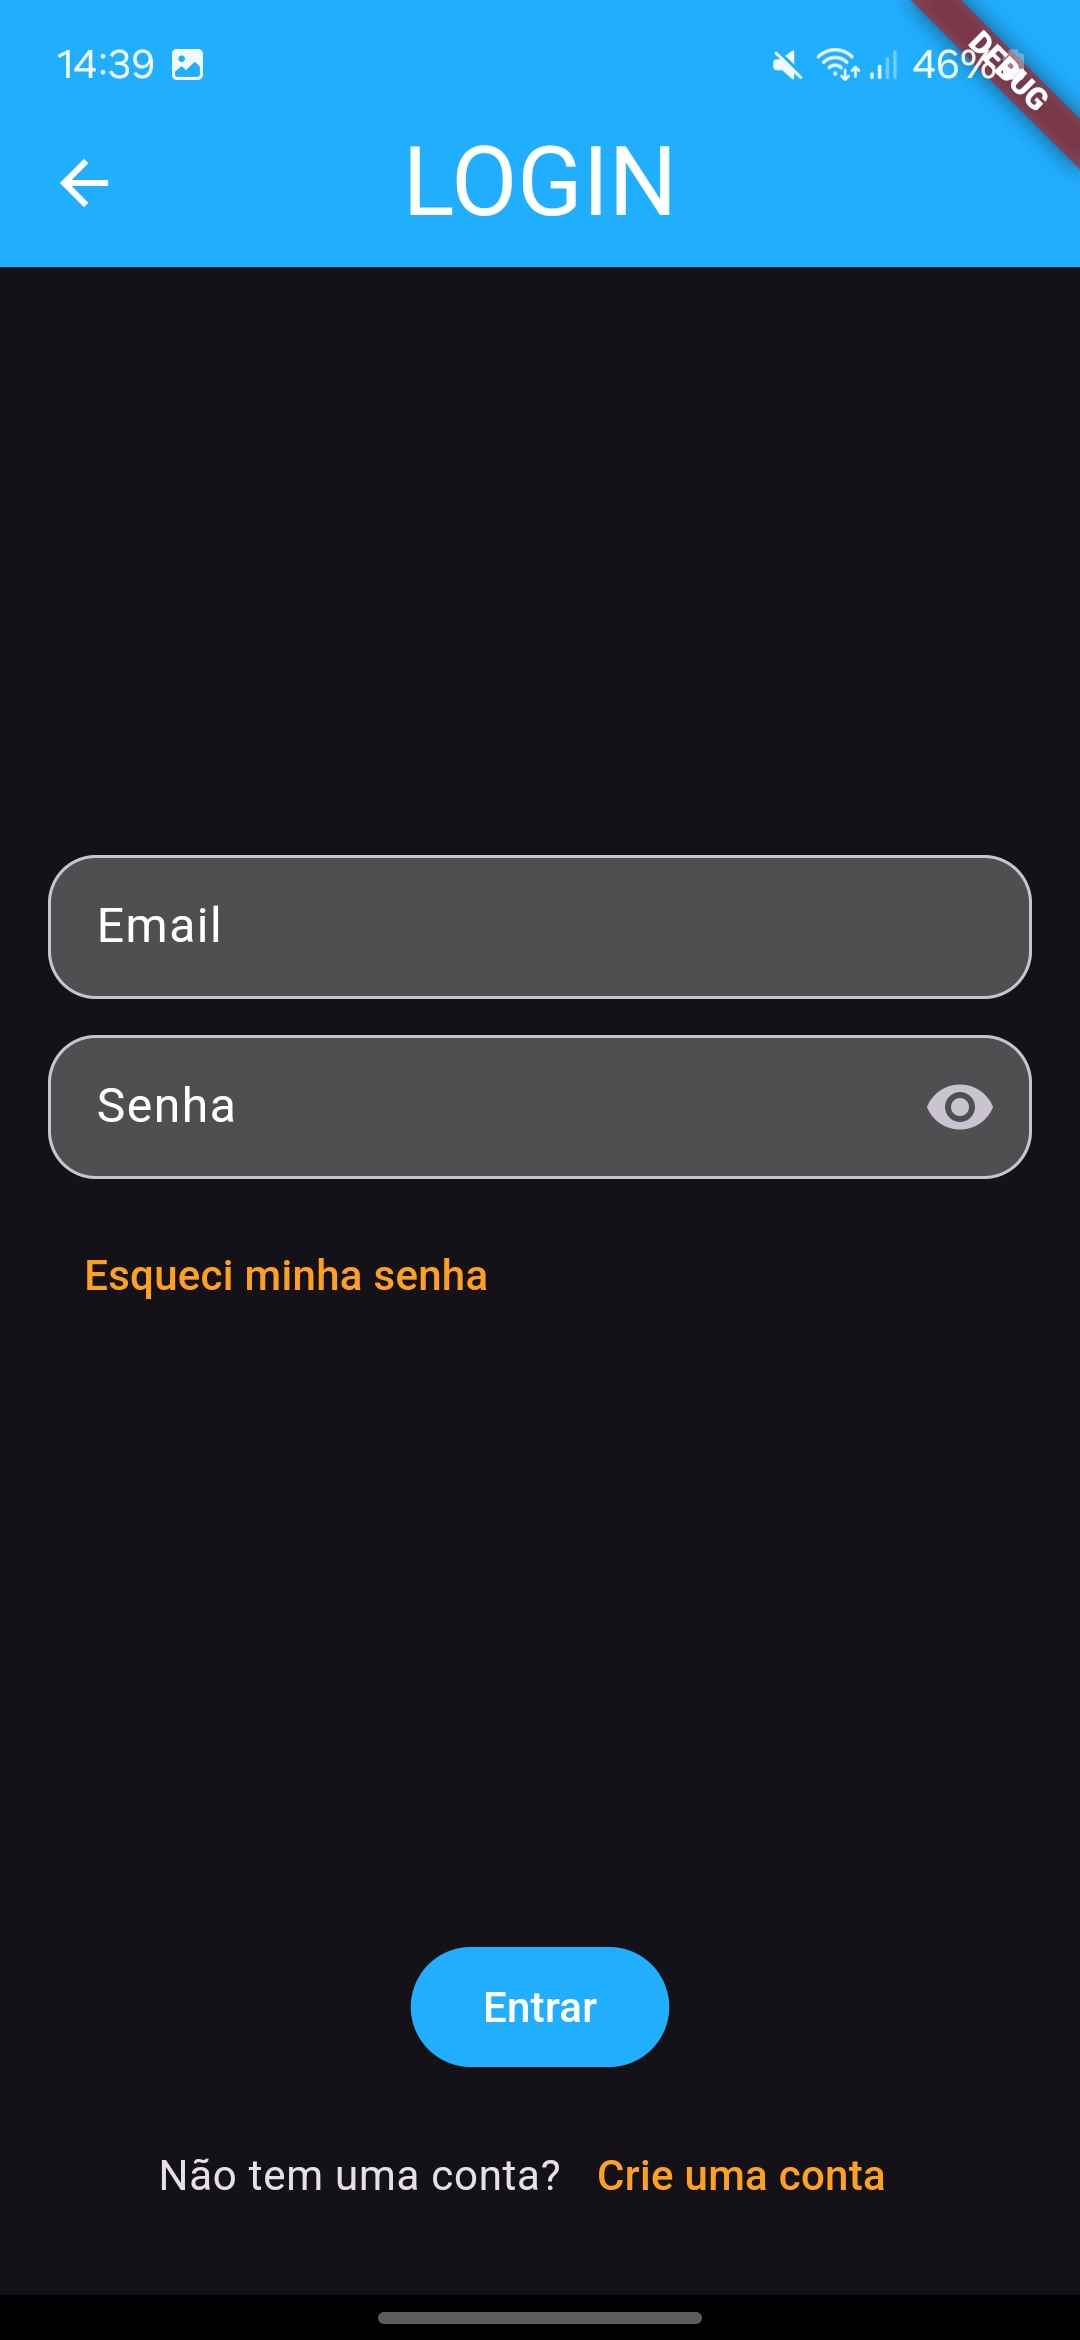
\includegraphics[width=44mm,height=80mm]{imagens/login.jpg}
        \hspace{10mm}
        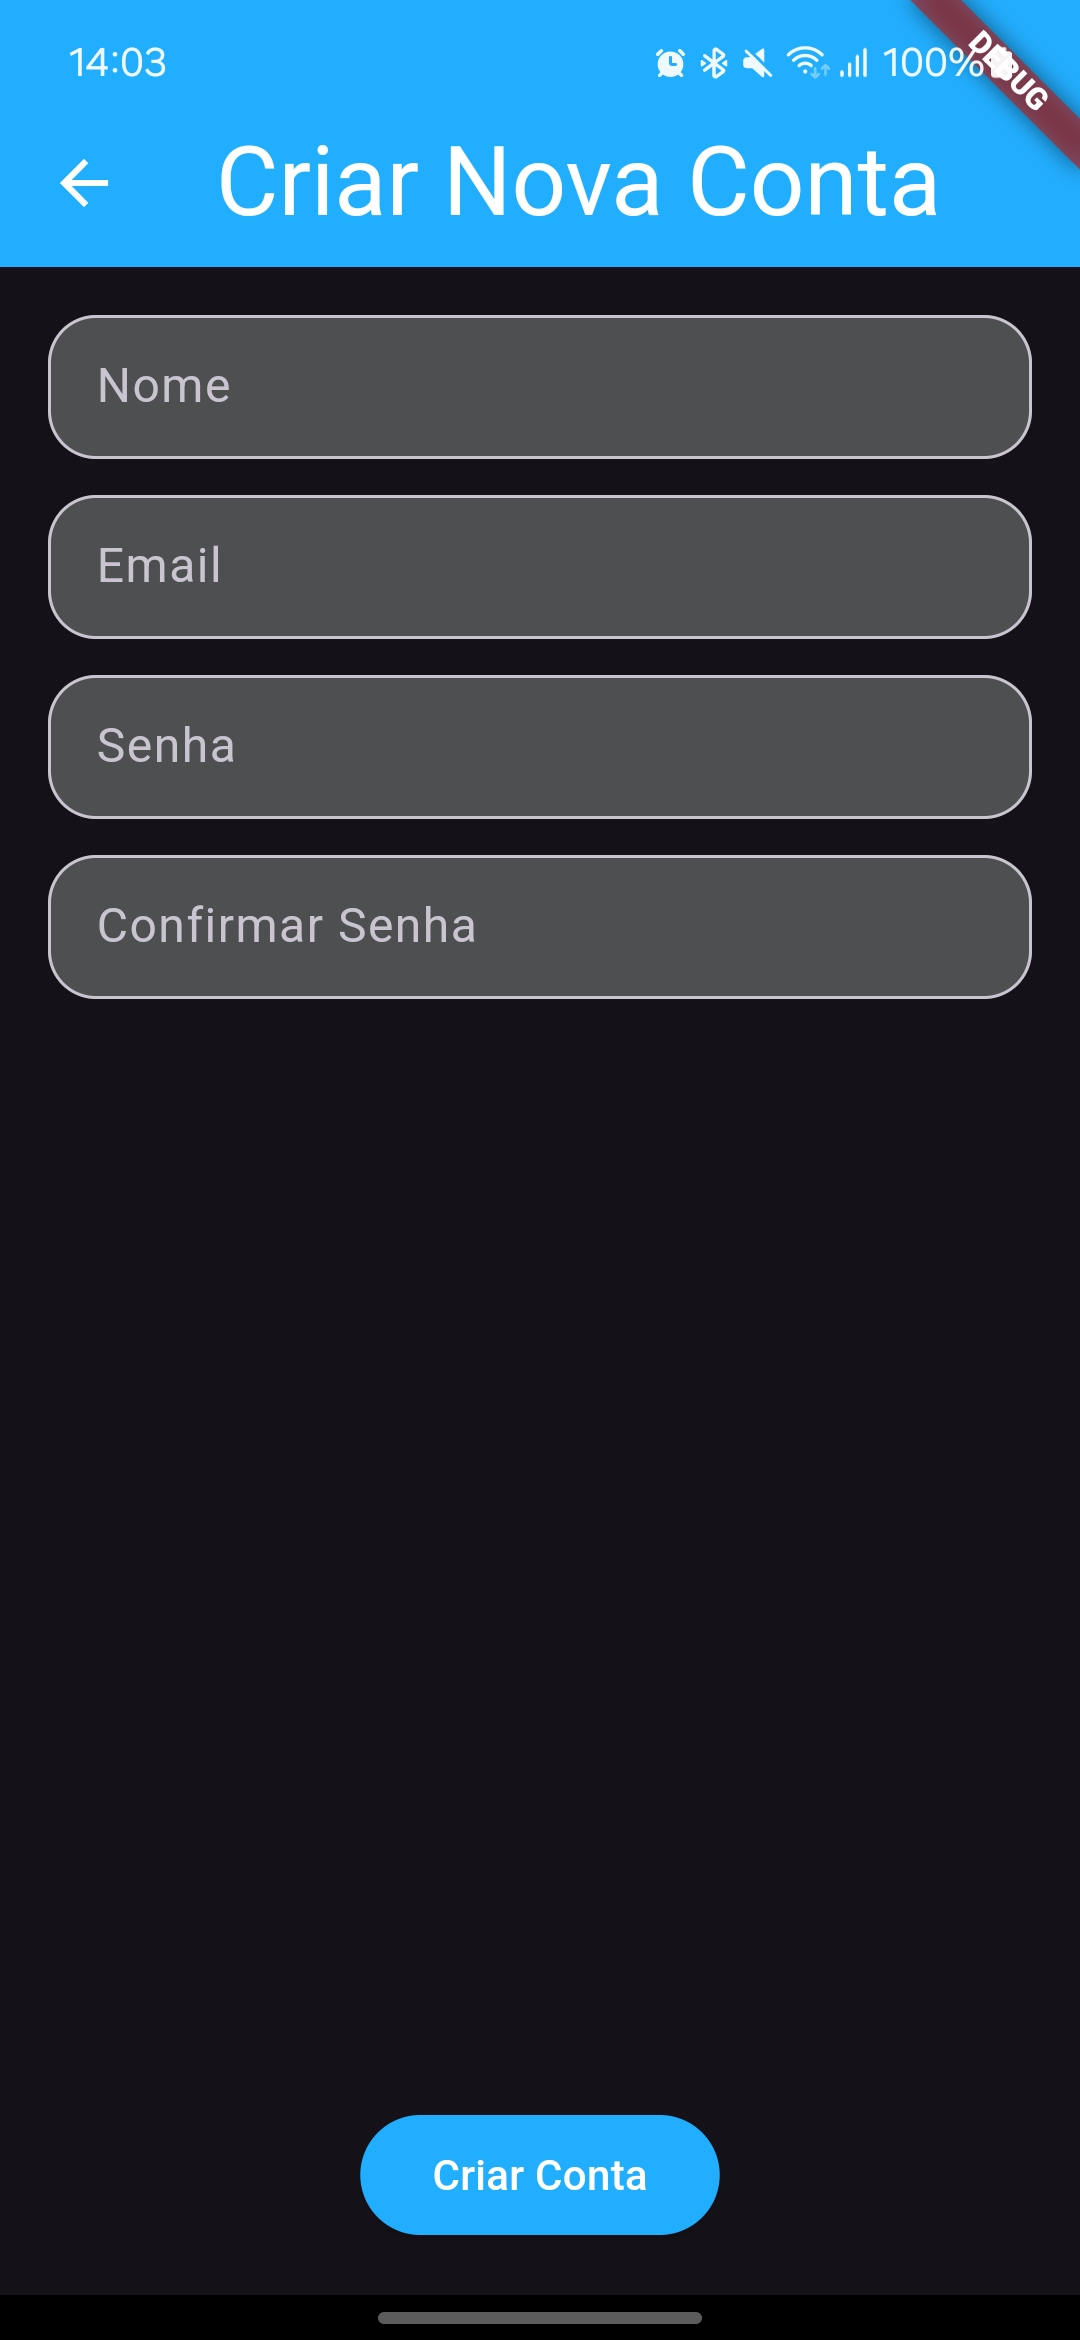
\includegraphics[width=44mm,height=80mm]{imagens/registrar.jpg} %tela de registro
        \caption{\scriptsize Tela 7: Login}
        \label{fig:tela7}
    \end{figure}

    \FloatBarrier
    
    Caso o usuário entre no processo de recuperação de senha ele deverá informar o email cadastrado e um email será enviado com um código de recuperação, que deverá ser informado numa tela subsequente, caso a verificação seja bem sucedida o usuário poderá definir uma nova senha. A Figura 12 mostra as telas de recuperação de senha.
    
    \FloatBarrier

    \begin{figure}[h]
        \centering
        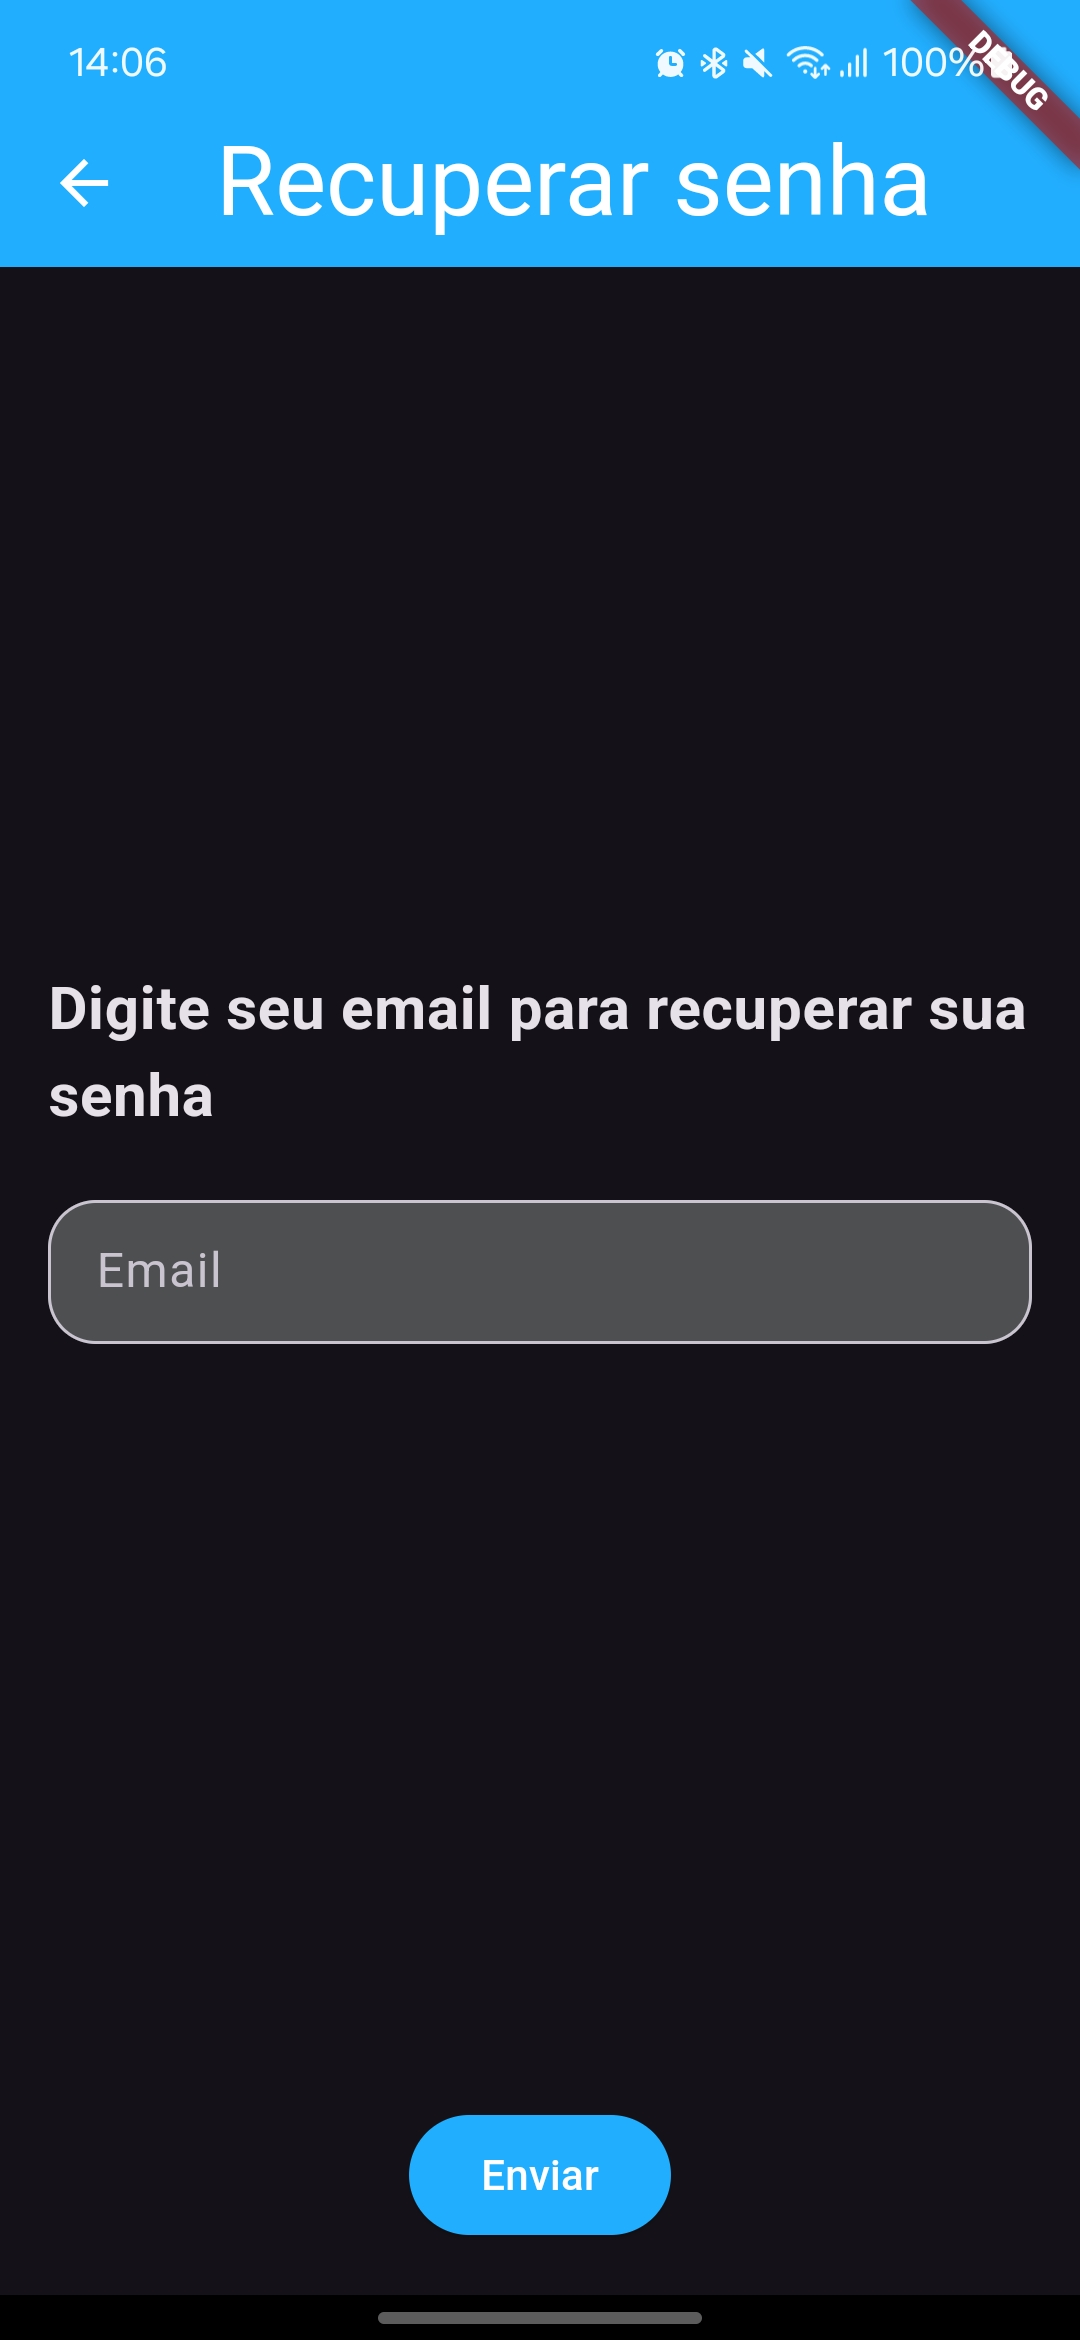
\includegraphics[width=44mm,height=80mm]{imagens/email.jpg} %tela de email
        \hspace{10mm}
        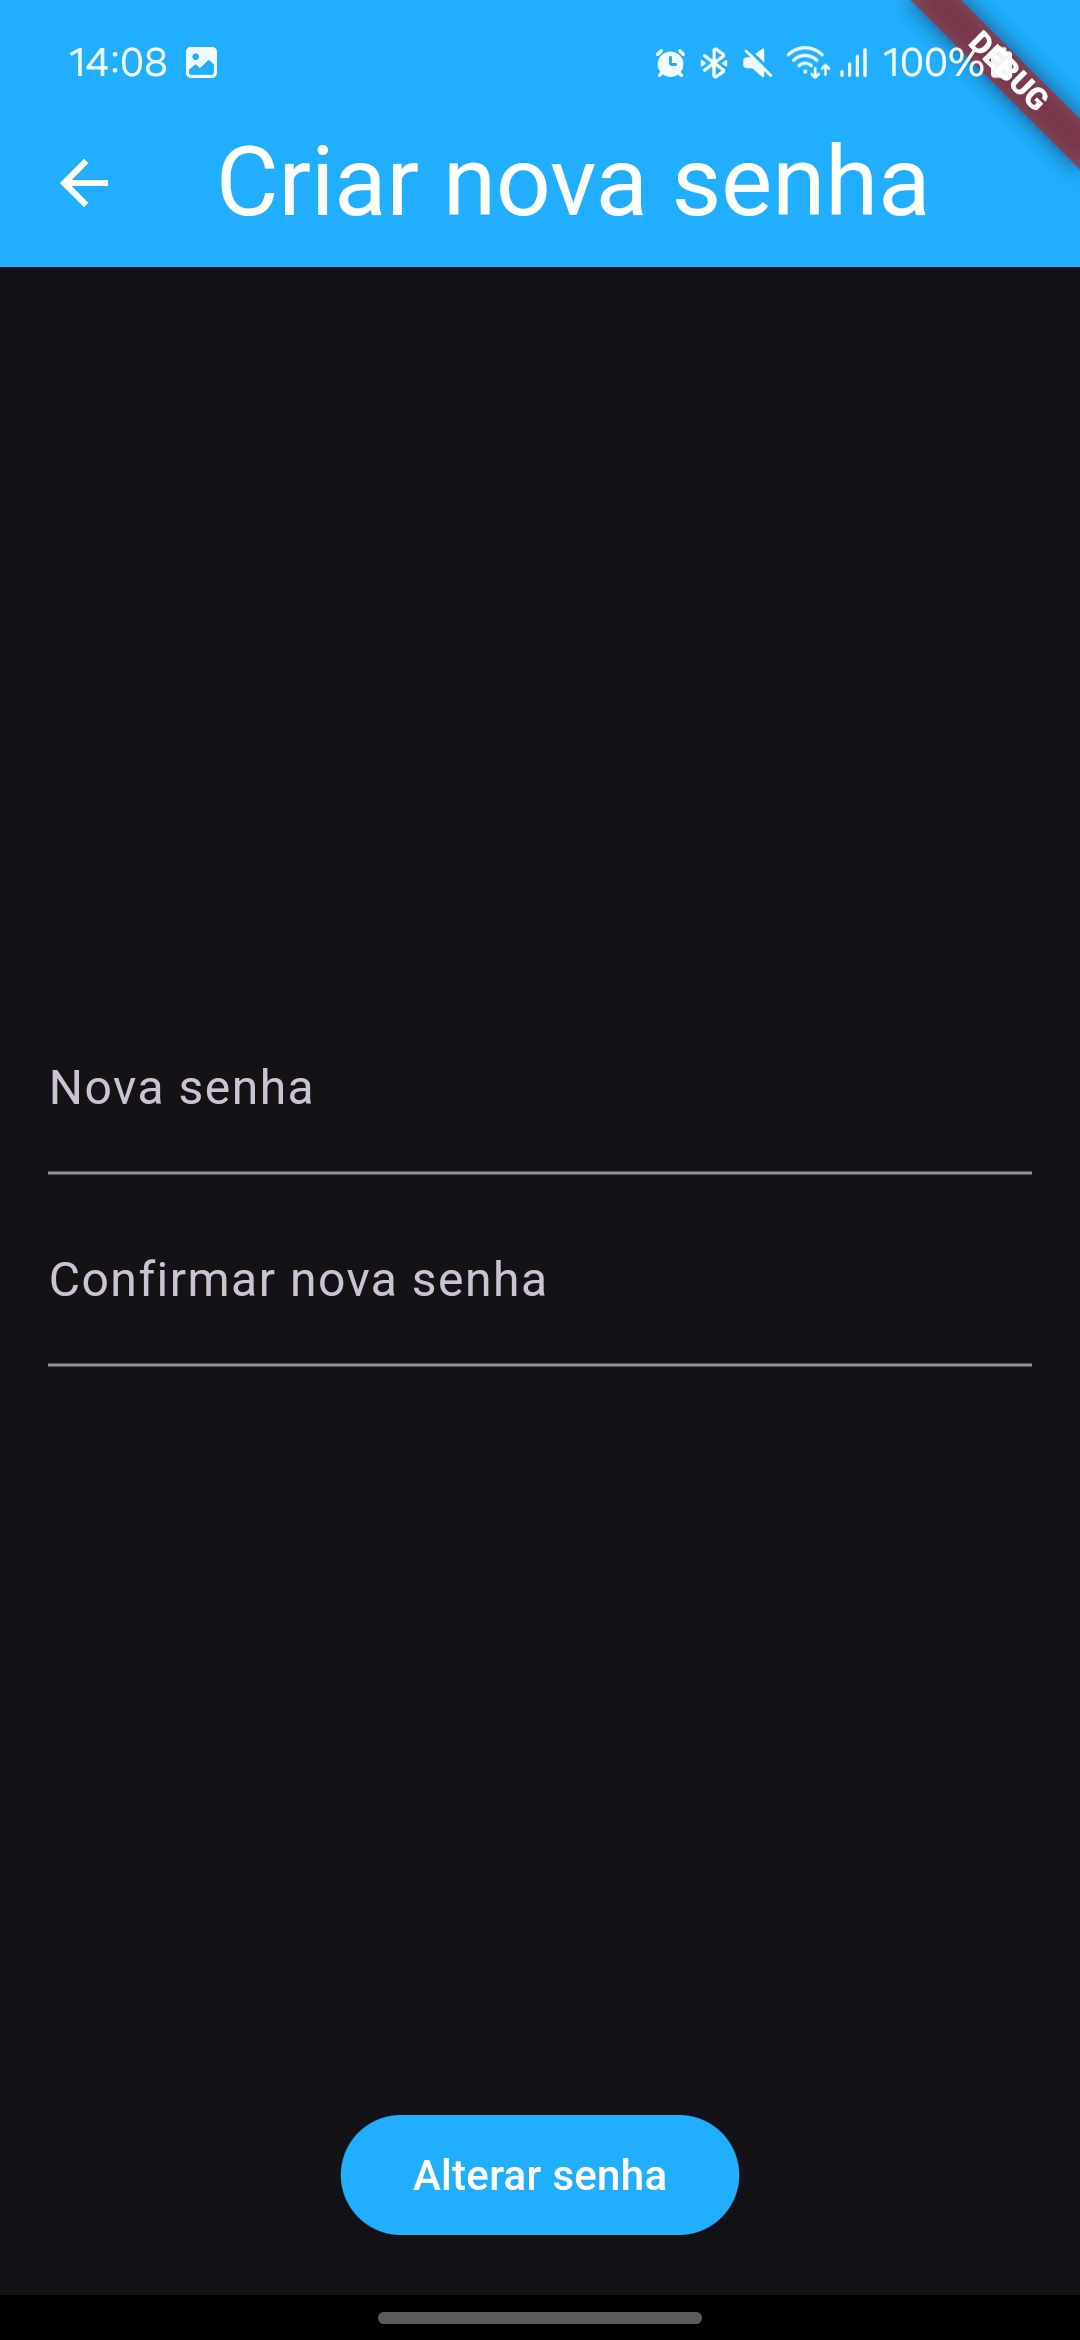
\includegraphics[width=44mm,height=80mm]{imagens/nova-senha.jpg} %tela de codigo
        \caption{\scriptsize Tela 7: Login}
        \label{fig:tela7-recuperacao}
    \end{figure}

    \FloatBarrier